\documentclass{article}
\usepackage{amsmath}
\usepackage{amssymb}
\DeclareMathOperator{\sign}{sign}
\usepackage{geometry}
\usepackage{subcaption}
\usepackage{standalone}
\usepackage{xcolor}
\usepackage{enumitem}
\setlist{nosep}

\usepackage{tikz}
\usetikzlibrary{patterns}
\usetikzlibrary{decorations.pathreplacing}

\usepackage{footnote}
\usepackage{csquotes}
\usepackage[USenglish]{babel}
\usepackage[backend=biber]{biblatex}

\addbibresource{articleBOS.bib}
\begin{document}
\today
\section{Abstract}

\section{Introduction}
The Background Oriented Schlieren technique (BOS) is an optical density visualization technique \cite{meier2002computerized,raffel2015background}. First described in \cite{dalziel2000whole}, where it was called Synthetic Schlieren (SS). This technique provides whole-field measurements of density gradients. One of the strengths of this technique was the simplicity of the experimental setup. Parts of the traditional, more extensive optical setups were replaced by digital image analysis. 

In a typical BOS or SS application, we image perturbations, or waves, traveling through a fluid. Two or more images are compared using Digital Image Correlation (DIC) [refs]. This comparison yields the displacements between the images. These displacements are related to the changes in the gradients of the index of refraction using a ray tracing model. These gradients of the index of refraction are related to the gradients of the density by experimentally determined data [refs], by the Gladstone-Dale relation for gases [refs] or by the Lorentz-Lorenz equation for liquids [refs]. The density field is sometimes obtained from the gradients of the density perturbations by solving a Poisson equation [refs].

In this paper we present a modification to the BOS or SS technique to directly measure the density field. We take images of static situations:  (1) before filling a tank in the experimental setup with (stratified) fluids, (2) after filling the tank with a calibration fluid and (3) after filling the tank with (stratified) fluids. Then we take images of the dynamic situations: we image, as in BOS or SS, the perturbations, or waves, traveling through a fluid. We perform DIC to obtain displacements between the static images. Using a ray tracing model we relate these displacements to the index of refraction. These static images give us the background index of refraction. We also perform DIC to obtain the displacements between the dynamic images and a static image.

The challenge of this new method was to have enough accuracy in our measurements and models to ensure that our results were useful. Determining the value of the density is more sensitive to noise than determining the density gradients of perturbations in a BOS or SS application. We also wanted to preserve the experimental simplicity of the BOS or SS method. In Section \ref{sec:simmod} we perform a naive application of the BOS or SS technique to try to measure the index of refraction of homogeneous water. We analyze a simple ray tracing model to determine why our naive approach failed. We show that light rays, traveling from the background through the fluid to the camera, should not travel in nearly straight lines (as in BOS or SS) but should have large deflections. We should either rotate the fluid tank or rotate (and move) our camera. We should not be placing our camera right in front of the fluid tank. 

To obtain the required accuracy in determining the density field we optimized all the steps in our method. In Section \ref{sec:formod} we derive our ray tracing model relating displacements to the index of refraction. We call this our forward model: given an index of refraction field and experimental parameters, we can compute the displacement field of our experimental setup. This ray tracing model is a 3D model that allows the camera to be placed under an angle with respect to the fluid tank. In Section \ref{sec:cal} we describe our calibration procedure. This calibration step allows us to determine very accurately certain parameters in our forward model.  In Section \ref{sec:DIC} we discuss DIC. We provide references to papers that discuss techniques that allowed us to get the most of our DIC procedure. We also provide information about our settings for a typical DIC calculation. In Section \ref{sec:exp} we briefly discuss the experimental setup. We also discuss best practices to get the most out of our experiments. In Section \ref{sec:invmod} we discuss how to solve our inverse model: how to obtain the index of refraction from the experimentally obtained displacements and our forward model. 

The two novel critical steps are: (1) To view the experimental setup under an angle and (2) To calibrate our model. 

\section{Simple Model}
\label{sec:simmod}
Consider the experimental set up as shown in Figure \ref{fig:schviepalira}. Light rays travel from a camera, through a water tank onto a background with a random dot pattern.  We describe the camera as a pinhole camera. We place the origin of the Cartesian coordinate system at the pinhole, the location where all light rays falling on the ccd sensor pass through. The $z$-axis is perpendicular to the experimental setup, i.e. such that a light ray traveling along the z-axis will not be refracted by the set-up. We want to determine the position where the light rays ends up, $x_6$. The light ray exits the camera with a position $x_1 = 0$ and an angle $\theta_x$. %The $x$-axis points opposite to gravity.

%\begin{figure}[hpbt]
%	\includestandalone{simplesetup}
%	\caption{A schematic view of a path of a light ray (not to scale). The numbers indicate the planes through which the light ray propagates: 1, the camera lens; 2, the start of the first glass plate; 3, the end of the first glass plate; 4, the start of the second glass plate; 5, the end of the second glass plate; 6, the screen from which the light rays originate. $n_0$, $n_1$ and $n_2$ are the index of refraction of, respectively, air, material of the tank and the fluid. The lengths are: $L_c$, the distance from camera to the first glass plate; $L_g$, the width of the glass plates; $L_t$ the width of the tank; $L_s$, the distance from the second glass plate to the screen.}
%	\label{fig:schviepalira}
%\end{figure}

\begin{figure}[hpbt]
	\includestandalone{schematicsetupangle}
	\caption{A schematic view of a path of a light ray (not to scale). The light ray in the reference state is indicated by a solid line, the light ray after filling the tank with water by a dashed line. The numbers indicate the planes through which the light ray propagates: 0, the ccd sensor inside the camera; 1, the camera pinhole; 2, the start of the first glass plate; 3, the end of the first glass plate; 4, the start of the second glass plate; 5, the end of the second glass plate; 6, the screen from which the light rays originate.  $n_0$, $n_1$ and $n_2$ are the index of refraction of, respectively, air, material of the tank and the fluid. The lengths (in the $z$-direction) are: $L_c$, the distance from camera to the first glass plate; $L_g$, the width of the glass plates; $L_t$ the width of the tank; $L_s$, the distance from the second glass plate to the screen.}	
\label{fig:schviepalira}	
\end{figure}

Assuming the refractive index in each section of the set up is constant, we can write for the light path,
\begin{equation}
	\label{eq:simpleline}
x(z) = x_i + z \tan \theta_i, \qquad i = 1, ... , 5,
\end{equation}
where $x_i$ is the $x$-position of the light ray at the start of each section and $\theta_i$ is the angle between the direction the ray is propagating and the $z$-axis. When encountering a discontinuous change in refractive index (when passing between the sections), we invoke Snell's laws
\begin{equation}
	\label{eq:snellslaw}
n_i \sin \theta_i = \mbox{ constant},
\end{equation}
where $n_i$ is the refractive index for the $i^{th}$ section. The position $x_6$ is
\begin{align}
\label{eq:simplex6}
x_6 (\theta_x, n_2) & =  (L_c+L_s) \tan \theta_x + 2 L_g \tan \arcsin \frac{n_0}{n_1} \sin \theta_x + L_t \tan \arcsin \frac{n_0}{n_2} \sin \theta_x \nonumber \\
& =  (L_c+L_s) \tan \theta_x + \frac{2 L_g n_0 \sin \theta_x}{\sqrt{n_1^2 - n_0^2 \sin^2 \theta_x}} + \frac{L_t n_0 \sin \theta_x}{\sqrt{n_2^2 - n_0^2 \sin^2 \theta_x}}.
\end{align}
The displacement $\Delta x$ is the difference in position $x_6$ between the constant reference state, $n_2 = n_0$, and the unknown state $n_2=n$, 
\begin{align}
\label{eq:dexcon2}
\Delta x = x_6 (n_2 = n_0) - x_6 (n_2 = n) & = L_t \left[ \tan \theta_x - \tan \arcsin \frac{n_0}{n} \sin \theta_x\right] \nonumber \\
& = L_t \left[ \tan \theta_x - \frac{n_0 \sin \theta_x}{\sqrt{n^2 - n_0^2 \sin^2 \theta_x}} \right] .
\end{align}
Inverting this relation we obtain the unknown refractive index $n$ as a function of the displacement
\begin{equation}
\label{eq:invdexcon2}
n = \frac{n_0 \sin \theta_x}{\sin \arctan \left( \tan \theta_x - \frac{\Delta x}{L_t} \right)} = \frac{n_0 \sin(\theta_x)}{\tan(\theta_x)-\frac{\Delta x}{L_t}} \sqrt{1+\left(\tan(\theta_x)-\frac{\Delta x}{L_t}\right)^2}.
\end{equation}
The angle $\theta_x$, the displacement $\Delta x$ and unknown index of refraction $n$ are functions of the coordinate $x$. % Equation (\ref{eq:invdexcon2}) holds for each point. 

%The index of refraction of air $n_0$ is constant. The light ray hits the first glass plate with a position
%\begin{equation}
%\label{eq:tanlaw}
%x_2 = L_c \tan \theta_x.
%\end{equation}
%The index of refraction of the glass plate $n_1$ is constant. The angle under which the light ray propagates changes instantaneously, obeying Snell's law
%\begin{equation}
%\label{eq:snelllaw}
%n_0 \sin \theta_x = n_1 \sin \theta_T.
%\end{equation}
%For a constant index of refraction in the water tank $n_2$ the position $x_6$ is
%\begin{equation}
%x_6 (\theta_x, n_2) = (L_c+L_s) \tan \theta_x + 2 L_g \tan \arcsin \frac{n_0}{n_1} \sin \theta_x + L_t \tan \arcsin \frac{n_0}{n_2} \sin \theta_x
%\end{equation}
%The displacement $\Delta x$ is the difference in position $x_6$ for two different values of $n_2$. We take one known value, the %tank is filled with air, $n_0$, and one unknown value $n_2 = n$. 
%\begin{equation}
%\label{eq:dexcon2}
%\Delta x = x_6 (n_2 = n_0) - x_6 (n_2 = n) = L_t \left[ \tan \theta_x - \tan \arcsin \frac{n_0}{n} \sin \theta_x\right].
%\end{equation}
%We can invert this relation to obtain the unknown $n$,
%\begin{equation}
%\label{eq:nfromdxsimple}
%	n = \frac{n_0 \sin(\theta_x)}{\tan(\theta_x)-\frac{\Delta x}{L_t}} \sqrt{1+\left(\tan(\theta_x)-\frac{\Delta x}{L_t}\right)^2}.
%\end{equation}

Figure \ref{fig:simmod} shows the results when using (\ref{eq:invdexcon2}) to obtain the index of refraction $n$. We have two frontal images of the experimental setup; (1) Figure \ref{fig:air0simplefrontal}, without water, and (2) Figure \ref{fig:fresh0simplefrontal}, with water.  Applying a Digital Image Correlation (DIC) method we obtain (1) the correlation coefficient, a measure of the reliability of the method, (2) the horizontal displacements $\Delta x$, and (3) the vertical displacements $\Delta y$. Where coordinates where $\Delta x = 0$ and $\Delta y = 0$ are the location of the $z-axis$. We calculate the angles $\theta_x$ and $\theta_y$ with respect to this $z$-axis. Using (\ref{eq:invdexcon2}) we can compute the index of refraction $n$. Figure \ref{fig:nfromdxsimplefrontal} shows $n$ obtained from the horizontal displacements $\Delta x$.  Figure \ref{fig:nfromdysimplefrontal} shows $n$ obtained from the vertical displacements $\Delta y$. In Figure \ref{fig:nfrontal} we combine the horizontal and vertical displacements to obtain $n$.

\begin{figure}[htbp]
\begin{subfigure}{.45\linewidth}
		\centering 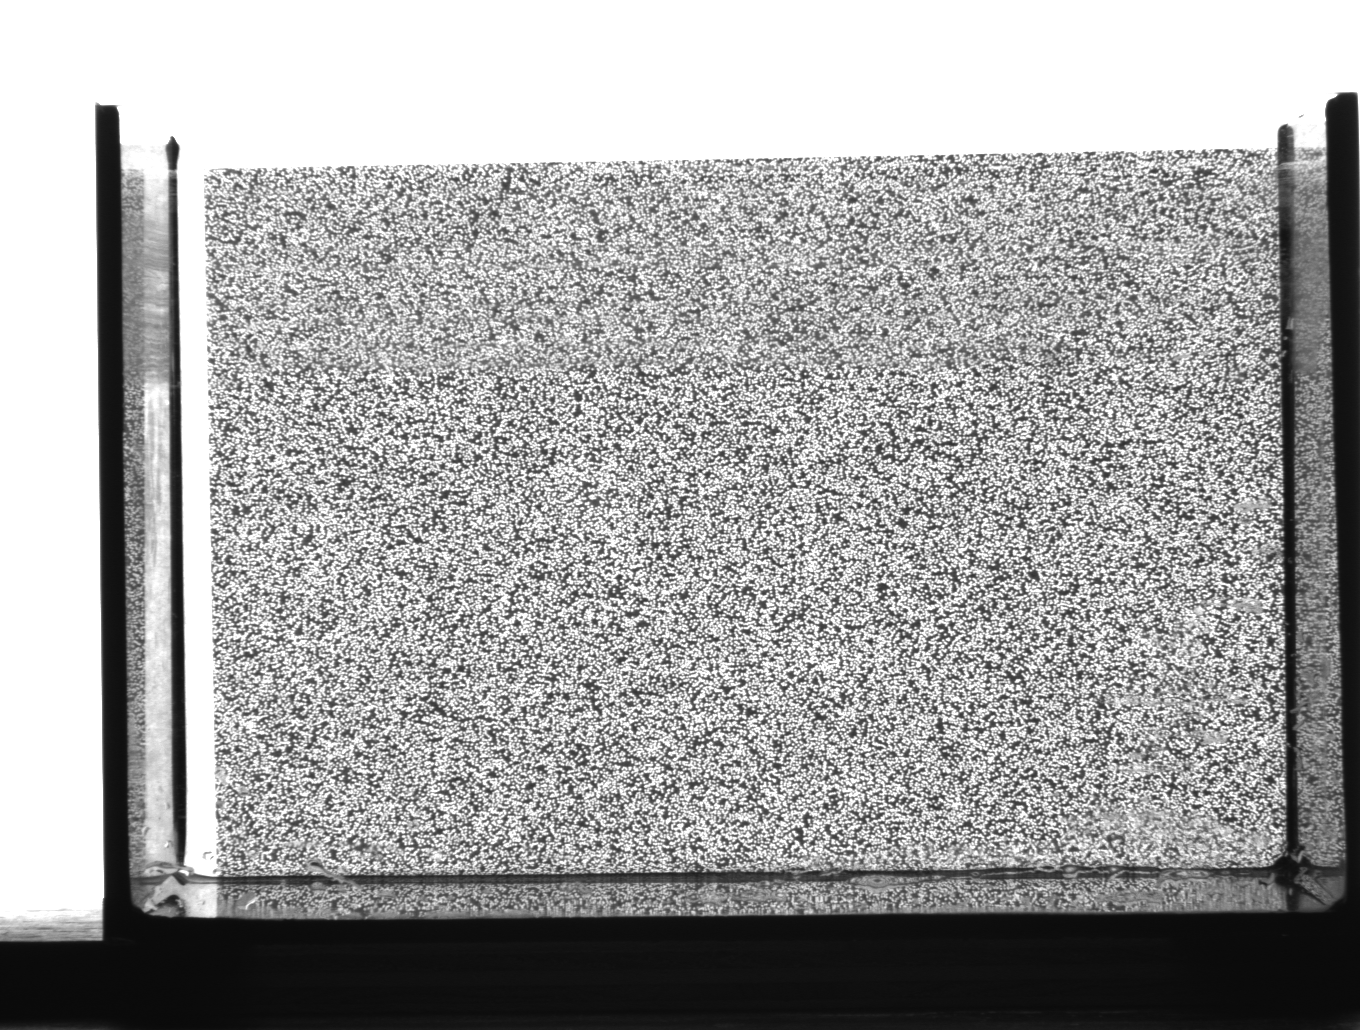
\includegraphics[width = \textwidth,keepaspectratio]{Refsimplefrontal}
		\subcaption{Reference Image: Filled with air}\label{fig:air0simplefrontal}
\end{subfigure}%
\begin{subfigure}{.45\linewidth}
	\centering 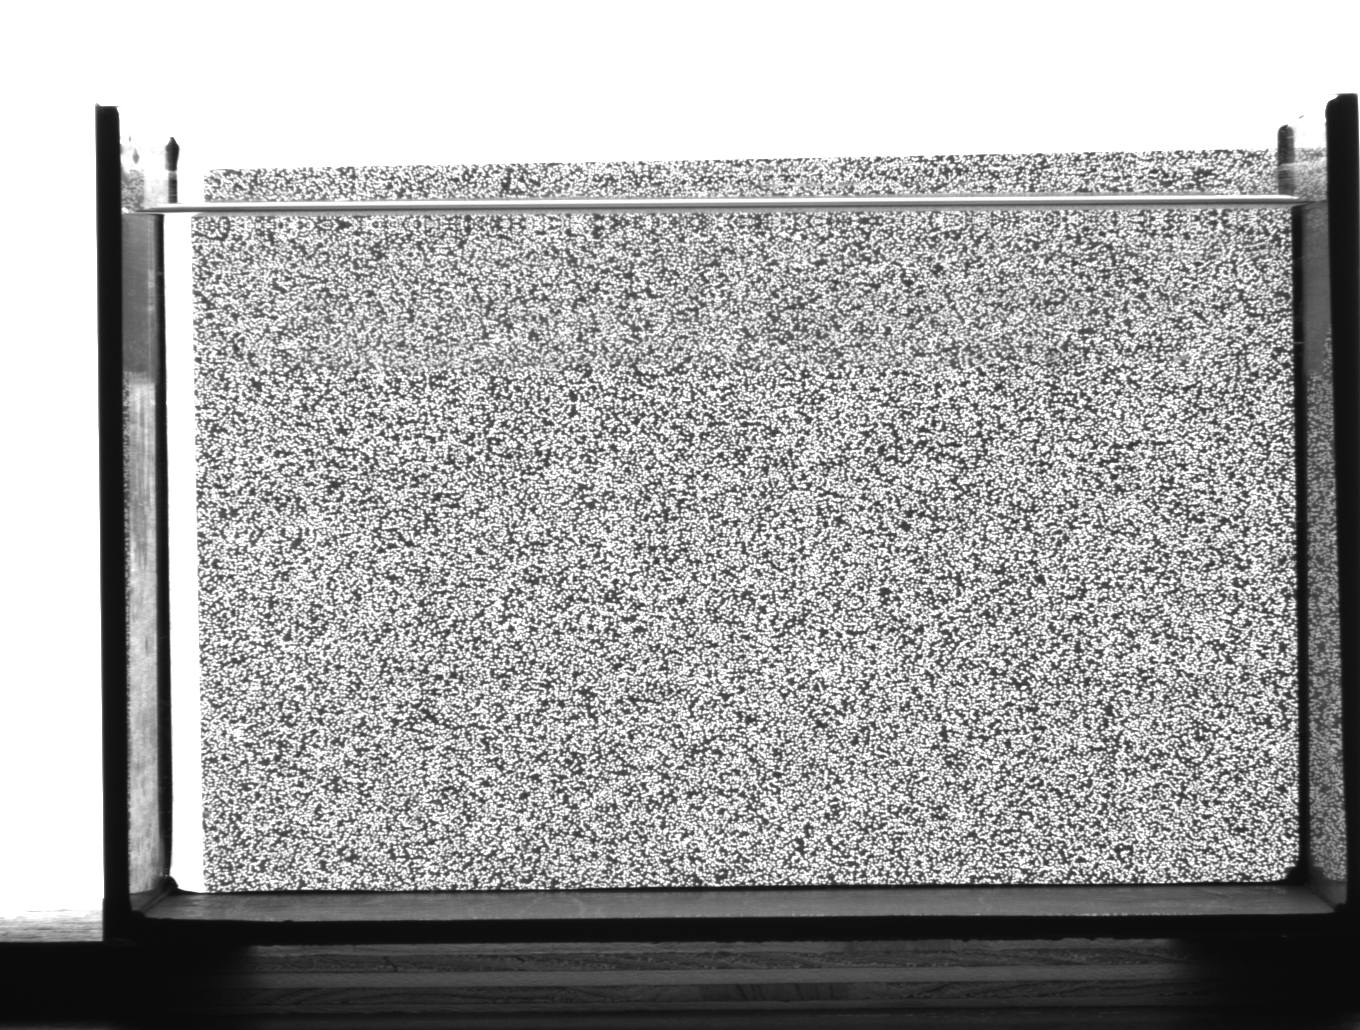
\includegraphics[width = \textwidth,keepaspectratio]{deformedsimplefrontal}
	\subcaption{Deformed Image: Filled with water}\label{fig:fresh0simplefrontal}
\end{subfigure}\\
\begin{subfigure}{.45\linewidth}
	\centering 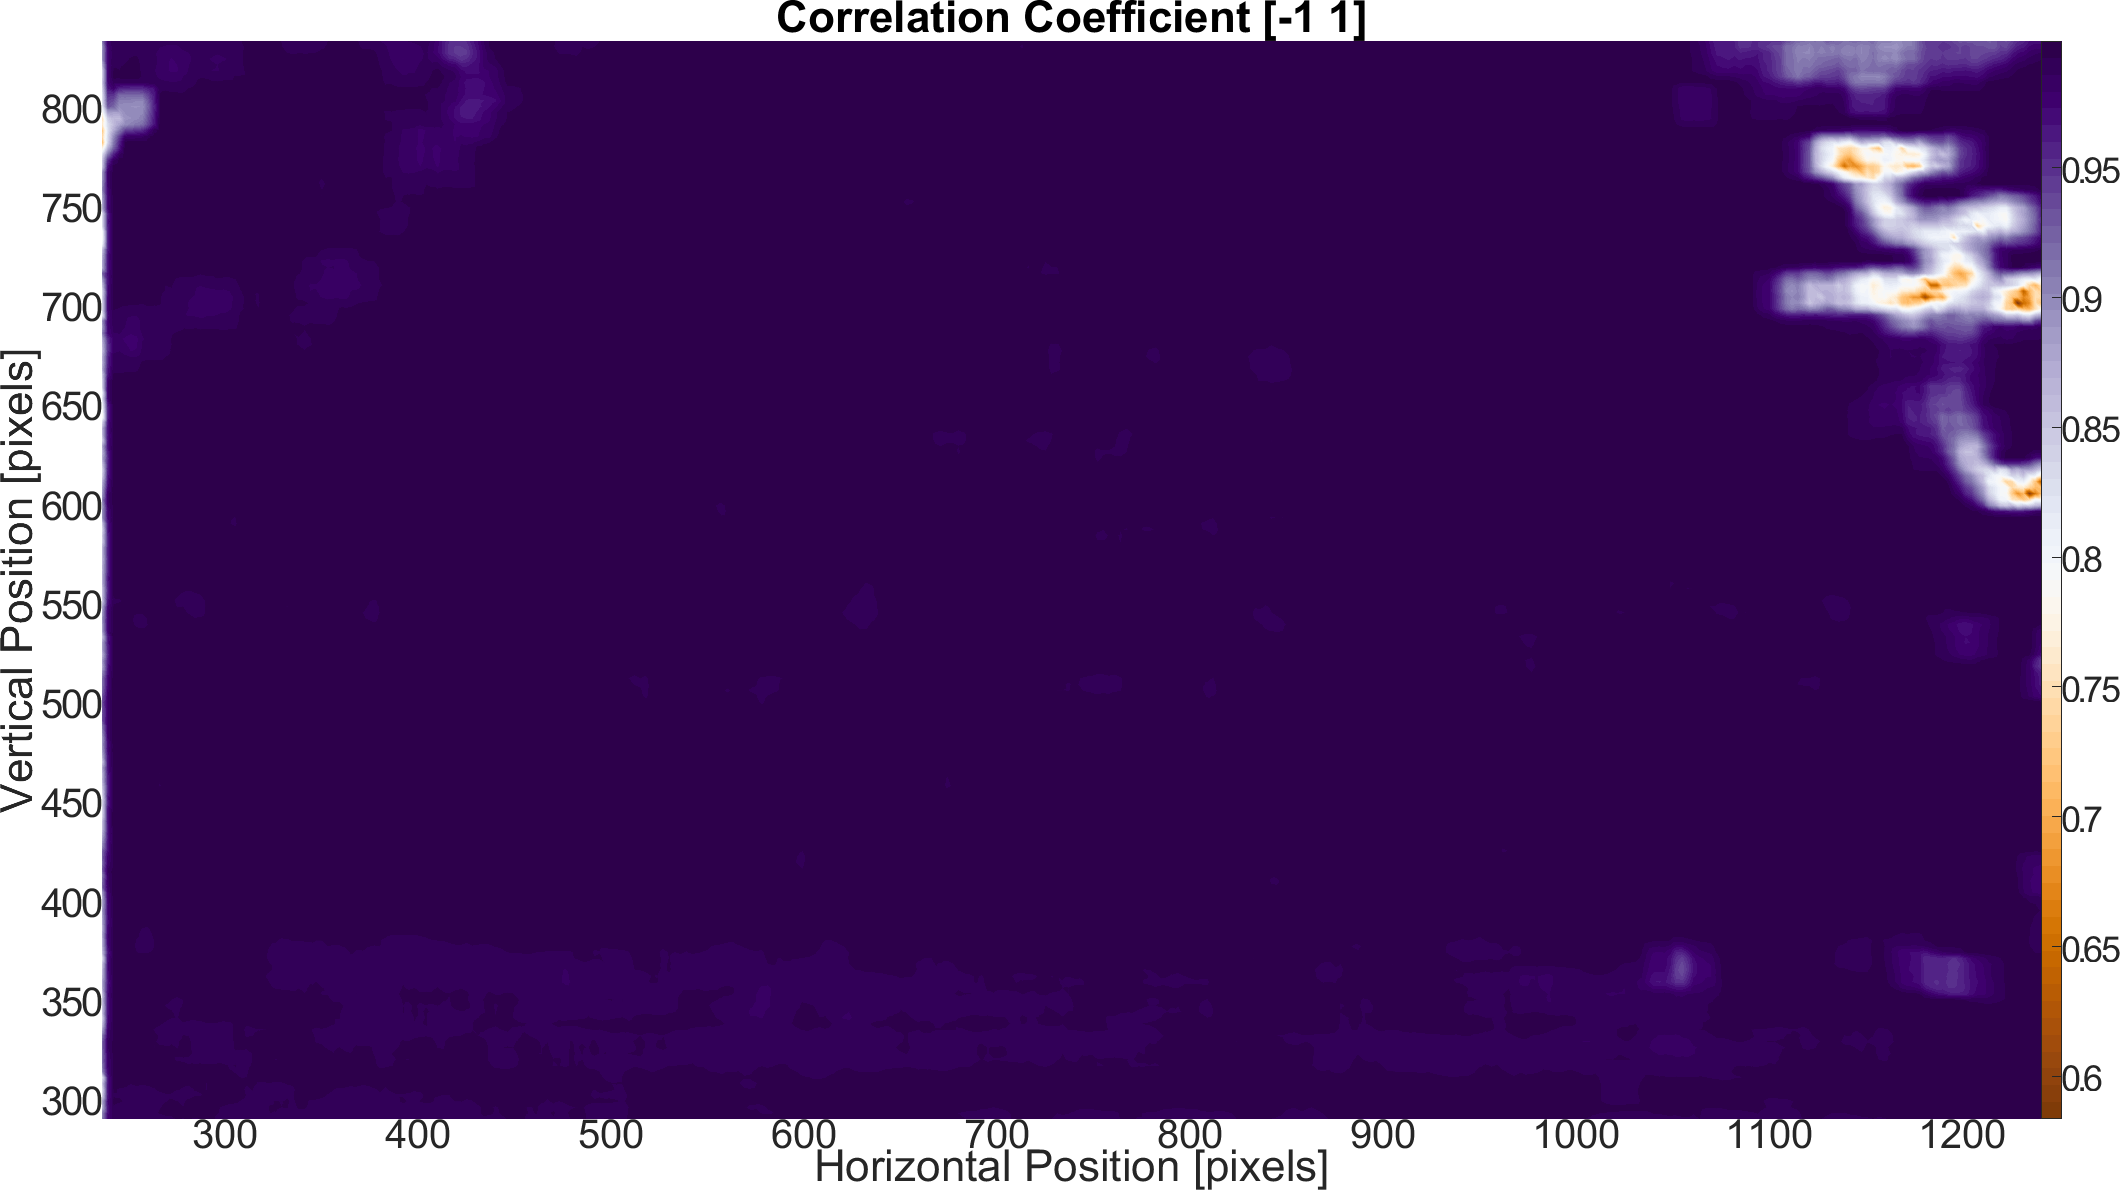
\includegraphics[width = \textwidth]{CCsimplefrontal}
	\subcaption{Correlation Coefficient from DIC}\label{fig:CCsimplefrontal}
\end{subfigure}%
\begin{subfigure}{.45\linewidth}
	\centering 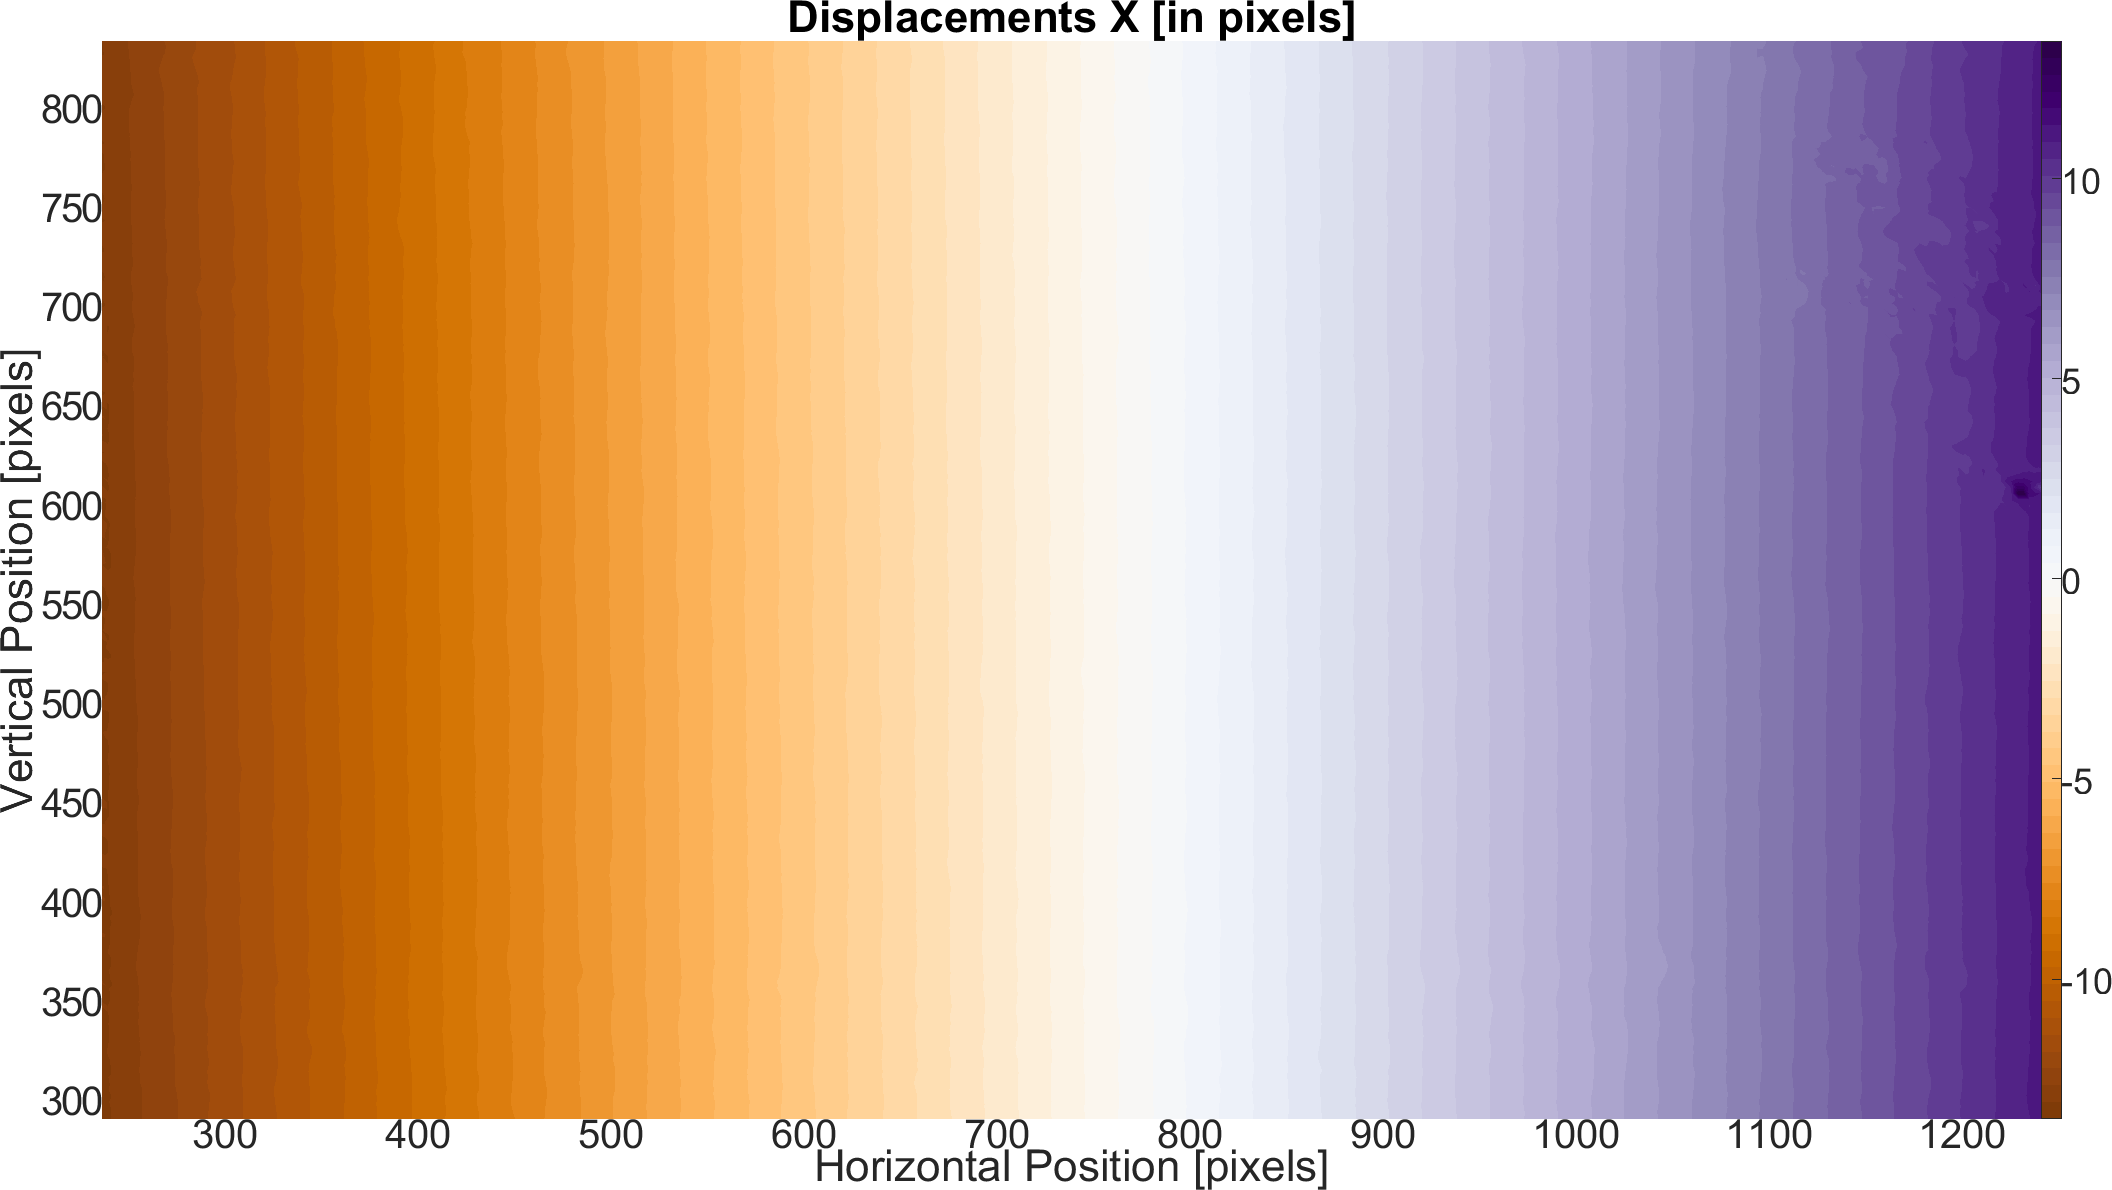
\includegraphics[width = \textwidth,keepaspectratio]{DXsimplefrontal}
	\subcaption{$\Delta x$ from DIC}\label{fig:DXsimplefrontal}
\end{subfigure}\\
	\begin{subfigure}{.45\linewidth}
	\centering 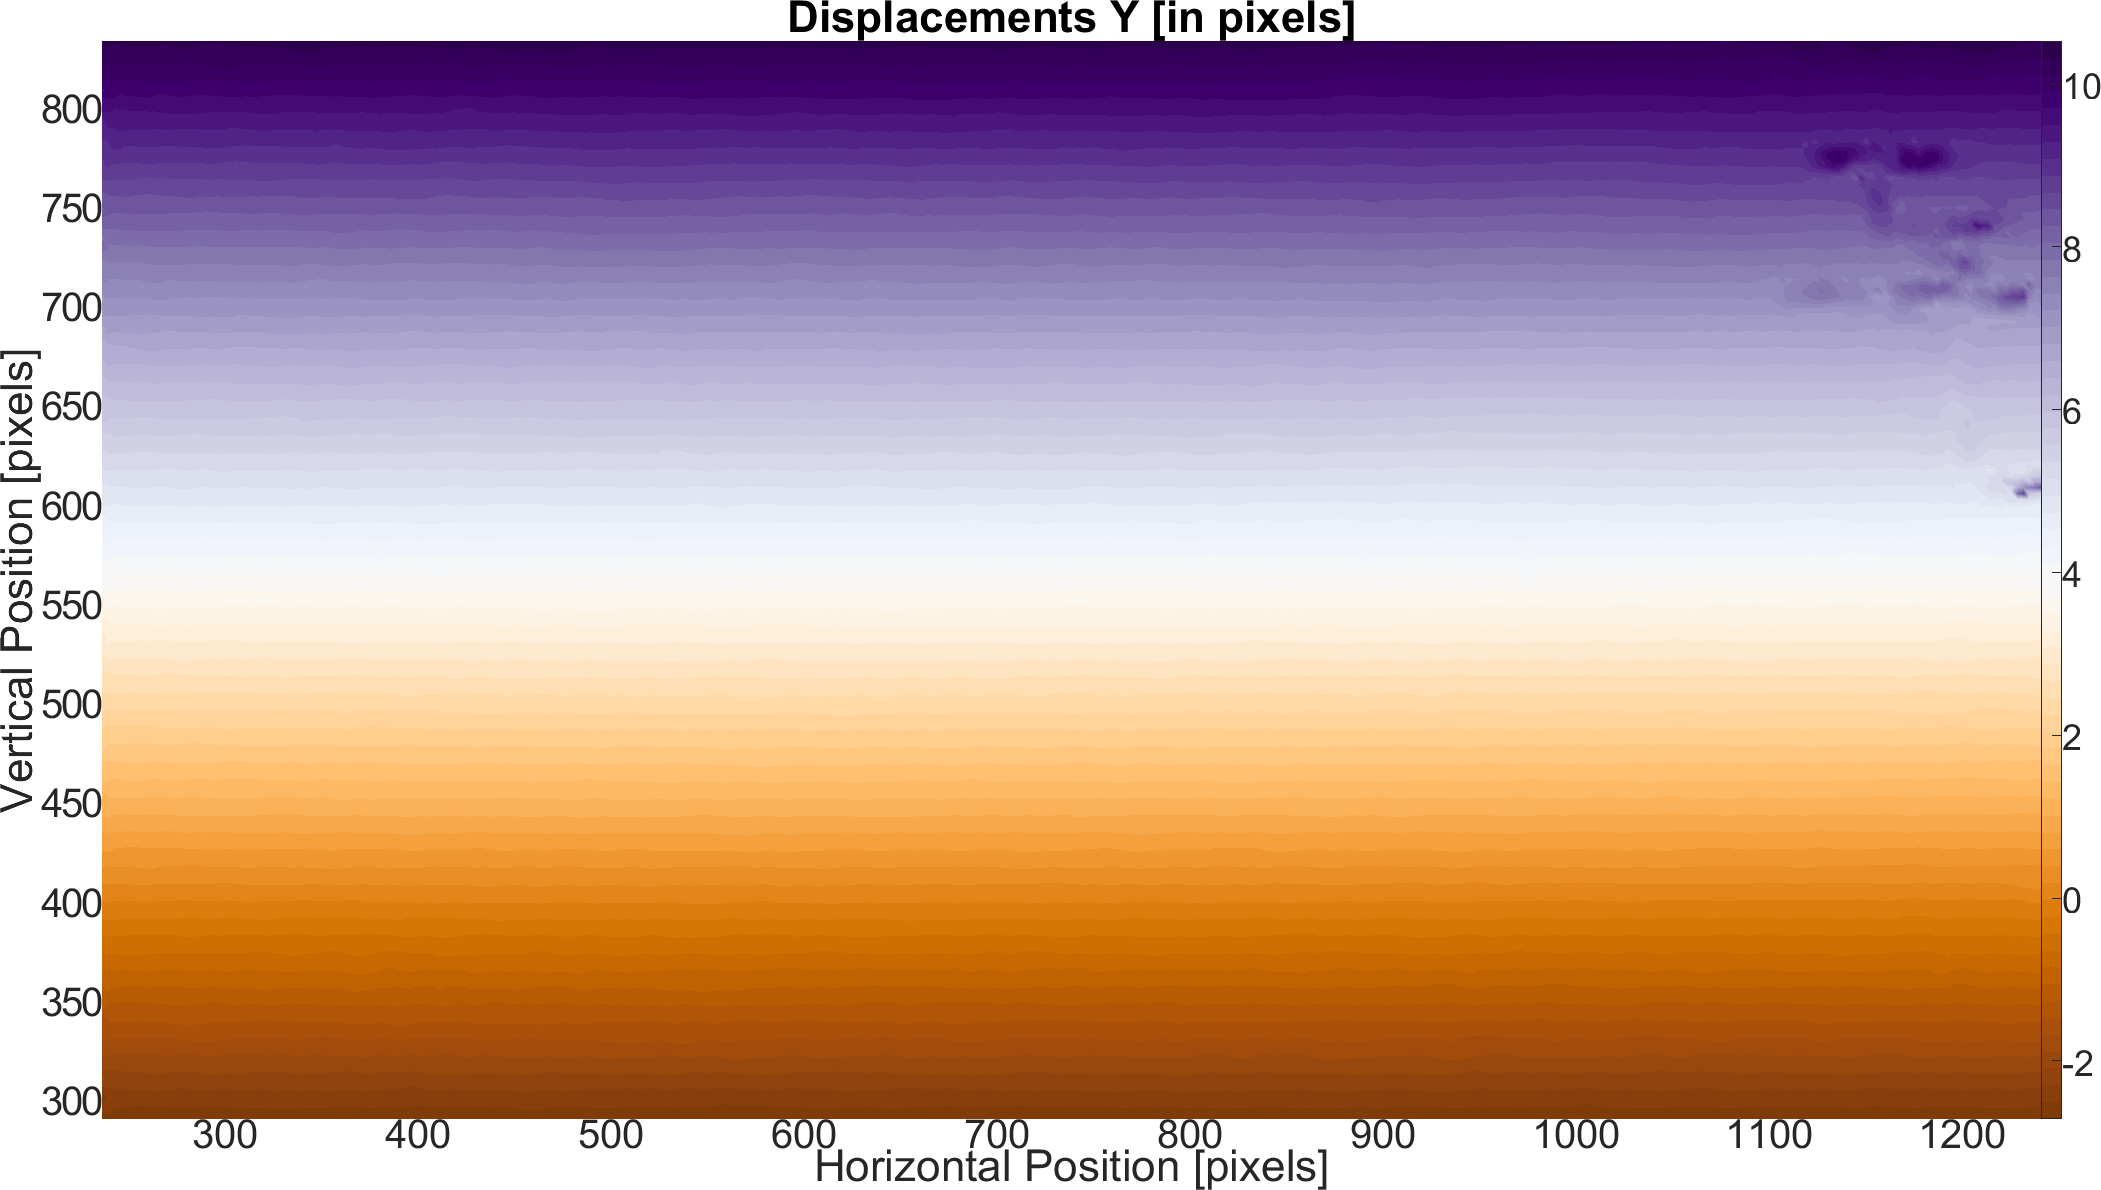
\includegraphics[width = \textwidth,keepaspectratio]{DYsimplefrontal}
	\subcaption{$\Delta y$ from DIC}\label{fig:DYsimplefrontal}
\end{subfigure}%
\begin{subfigure}{.45\linewidth}
	\centering 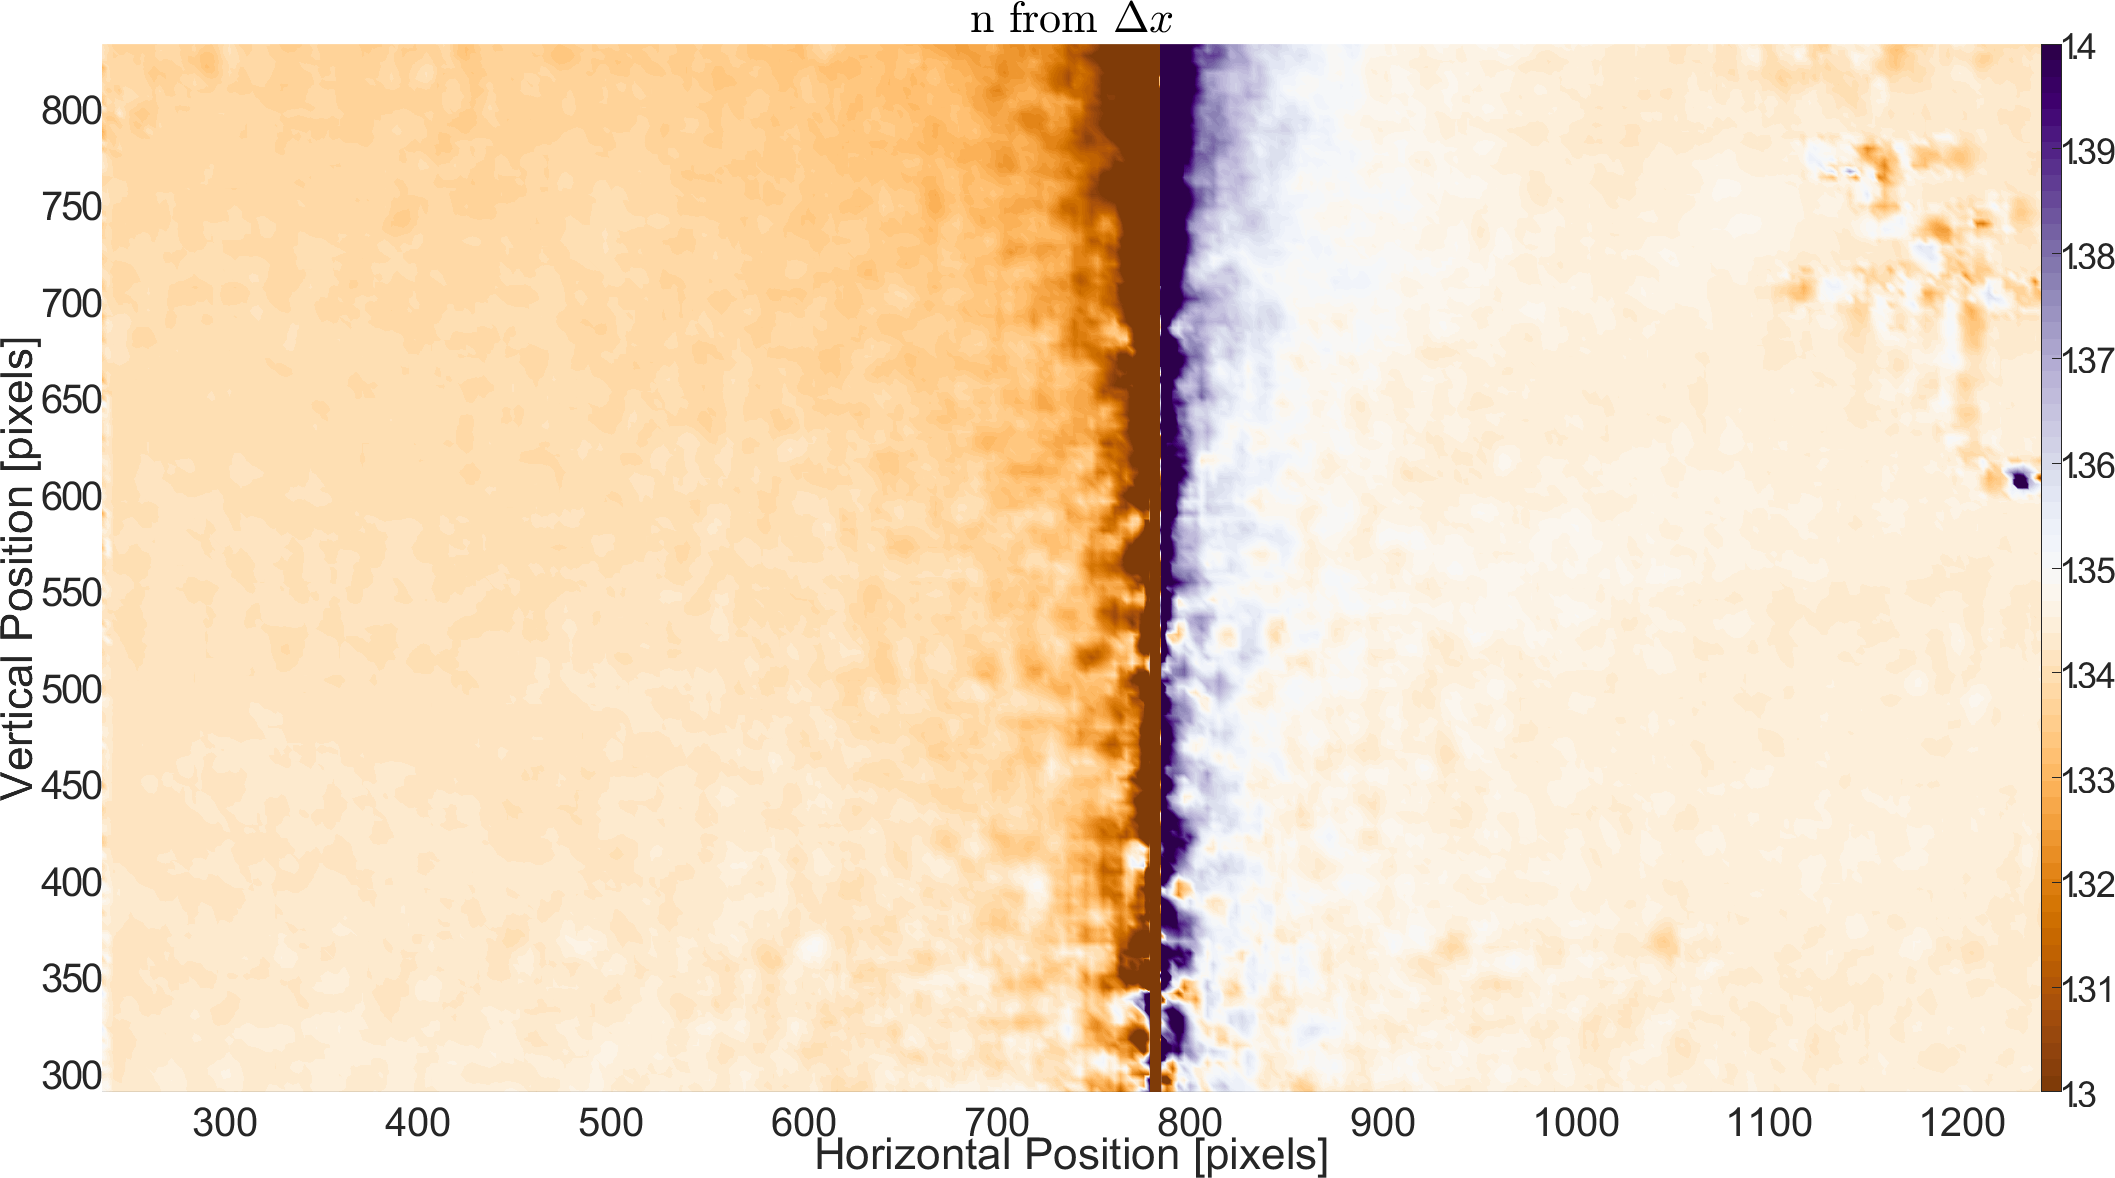
\includegraphics[width = \textwidth,keepaspectratio]{nfromdxsimplefrontal}
	\subcaption{$n$ from $\Delta x$}\label{fig:nfromdxsimplefrontal}
\end{subfigure}\\
\begin{subfigure}{.45\linewidth}
	\centering 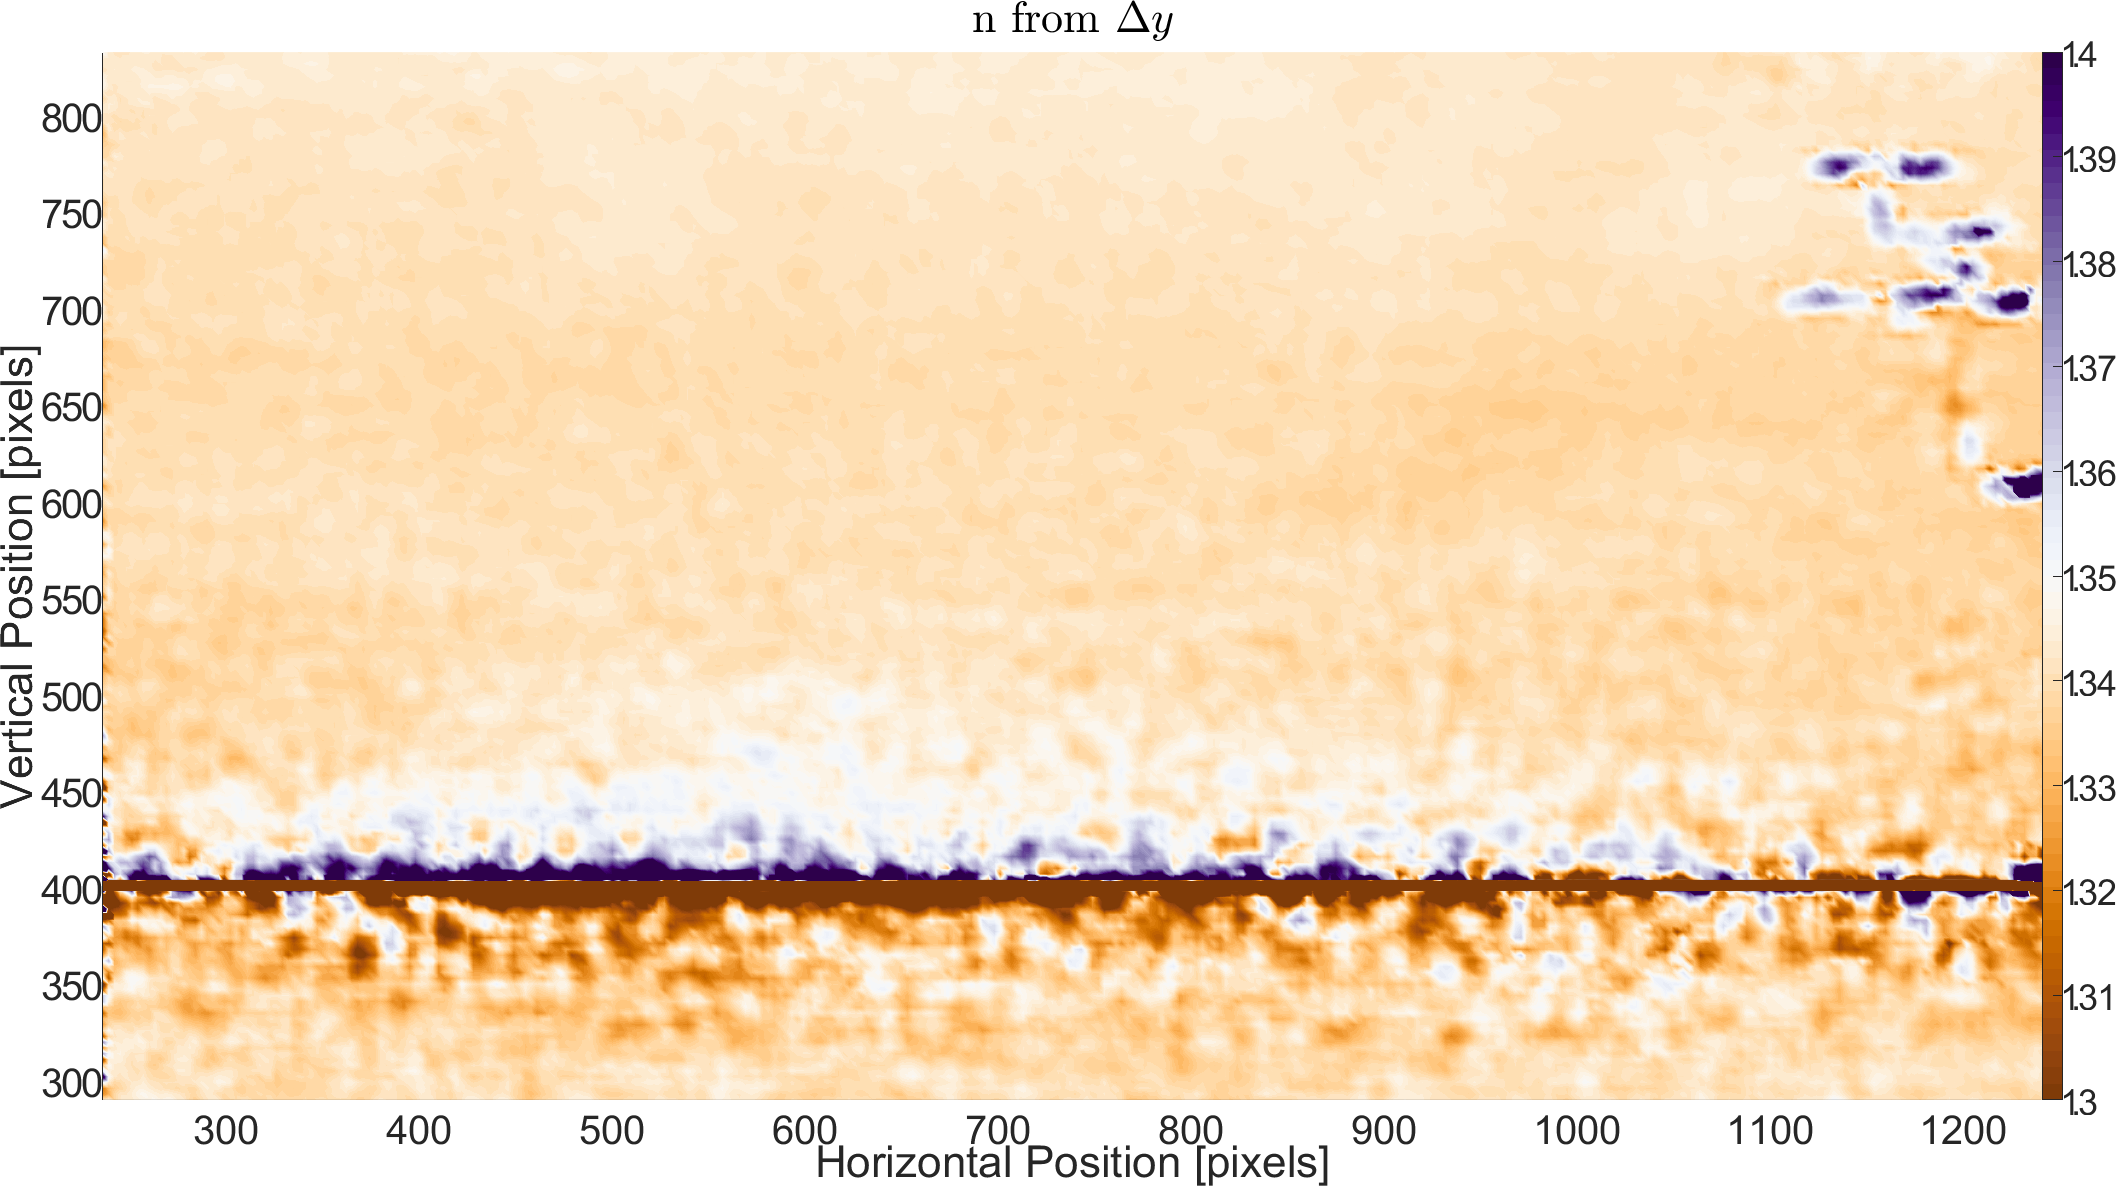
\includegraphics[width = \textwidth,keepaspectratio]{nfromdysimplefrontal}
	\subcaption{$n$ from $\Delta y$}\label{fig:nfromdysimplefrontal}
\end{subfigure}%
\begin{subfigure}{.45\linewidth}
	\centering 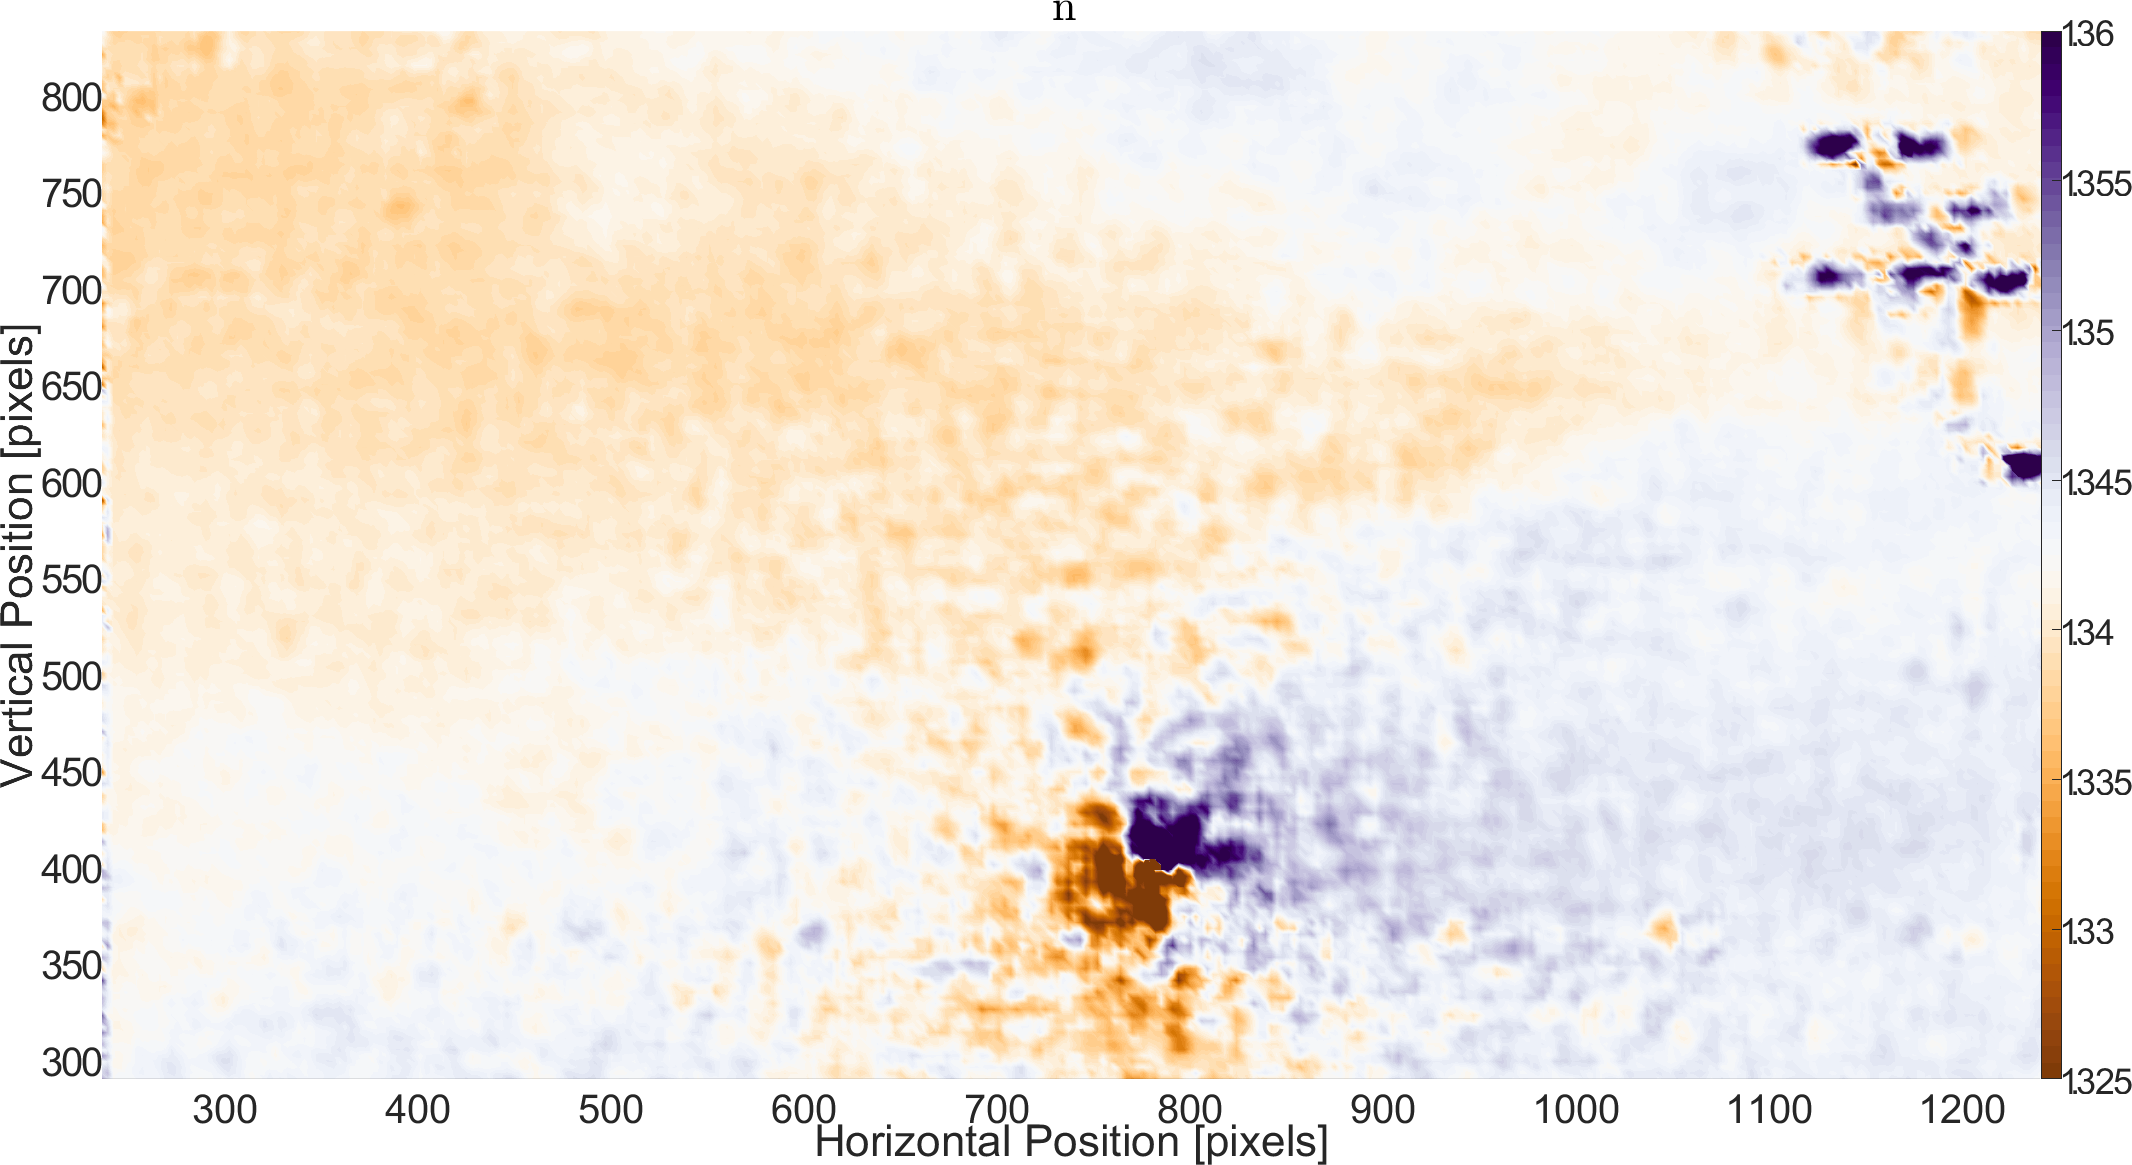
\includegraphics[width = \textwidth,keepaspectratio]{nsimplefrontal}
	\subcaption{$n$ from $\sqrt{\Delta x^2+\Delta y^2}$}\label{fig:nfrontal}
\end{subfigure}
\caption{Simple Model Result. When the angle $\theta_x$ is near zero, large errors in $n$ appear. }
\label{fig:simmod}
\end{figure}

We see that when the displacements approach zero, we have very large errors in $n$. Figure \ref{fig:nfrontal} looks best, but is still unacceptable. Around the location of the $z-axis$, where the angles and displacements approach zero, the errors are very large. The entire figure should have a constant value of $n = 1.333$. This is not the case.
 
Equations (\ref{eq:dexcon2}) and (\ref{eq:invdexcon2}) reveal a problem when determining $n$: When the angle $\theta_x$ goes to zero, (\ref{eq:dexcon2}) shows $\Delta x$ goes to zero. Then the numerator in the fraction in (\ref{eq:invdexcon2}) goes to zero, while the two terms in the denominator both go to zero. So we get large errors in the magnitude of $n$ since we are dividing $0/0$ and we get possibly negative values of $n$ since both terms in the denominator can go to zero. In any measurement we have noise, resulting in uncertainties in $\Delta x$ and $\theta_x$. These uncertainties have a large effect on the value of $n$ since the expected values of $\Delta x$ and $\theta_x$ are small. %The Signal-to-Noise Ratio is very bad because our signal is very small.

To solve this, we want $\theta_x$ to not approach zero. Then, according to (\ref{eq:dexcon2}), $\Delta x$ does not approach zero and our calculation of $n$ is not plagued by a fraction that approaches $0/0$. To achieve this, we place our camera at an angle $\alpha$ with respect to the water tank. The angle $\theta_x$ is replaced by $\alpha+\phi_x$, where $\phi_x$ is the angle of the light ray relative to the principal axis of the camera, which is at an angle $\alpha$. For example, we position our camera at an angle of $\alpha=30^\circ$ relative to the tank. The camera has a viewing range of $[-4,4]$ degrees. Then $\phi_x$ varies from $-4^\circ$ to $4^\circ$.

\begin{figure}[hpbt]
	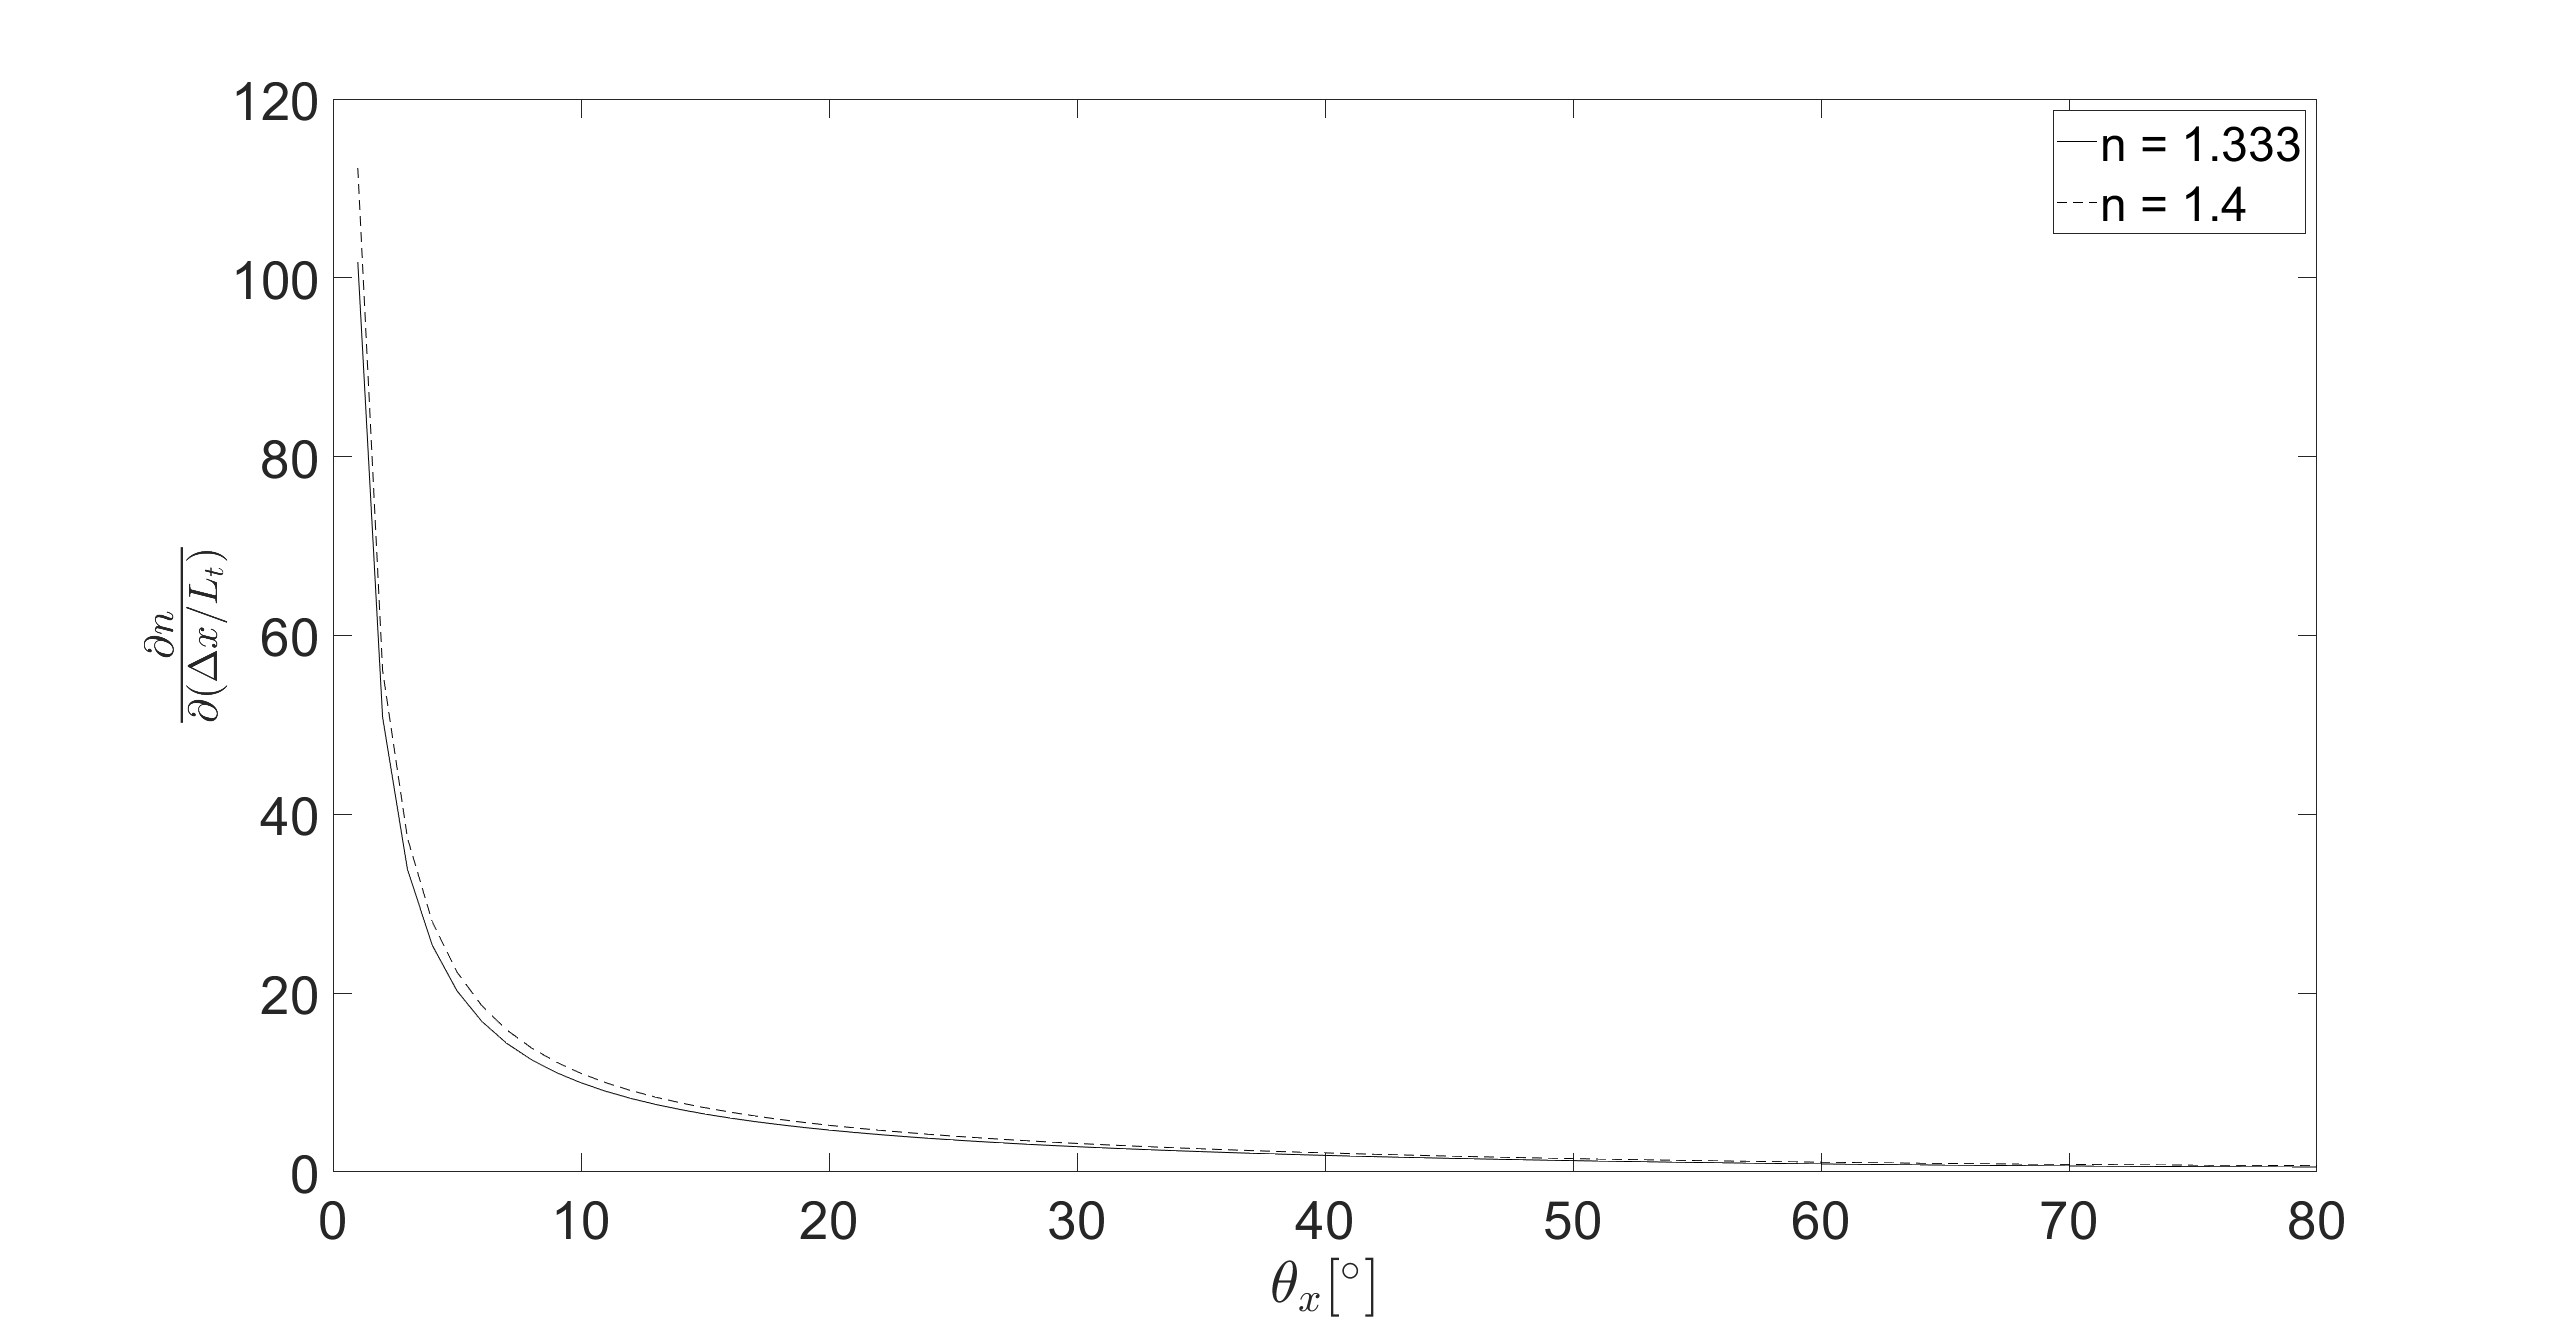
\includegraphics[width=\textwidth, keepaspectratio]{dndx.png}
	\caption{Derivative of $n$ with respect to $\Delta x / L_t$ as a function of $\theta_x$.}	
	\label{fig:dndx}
\end{figure}

\begin{figure}[hpbt]
	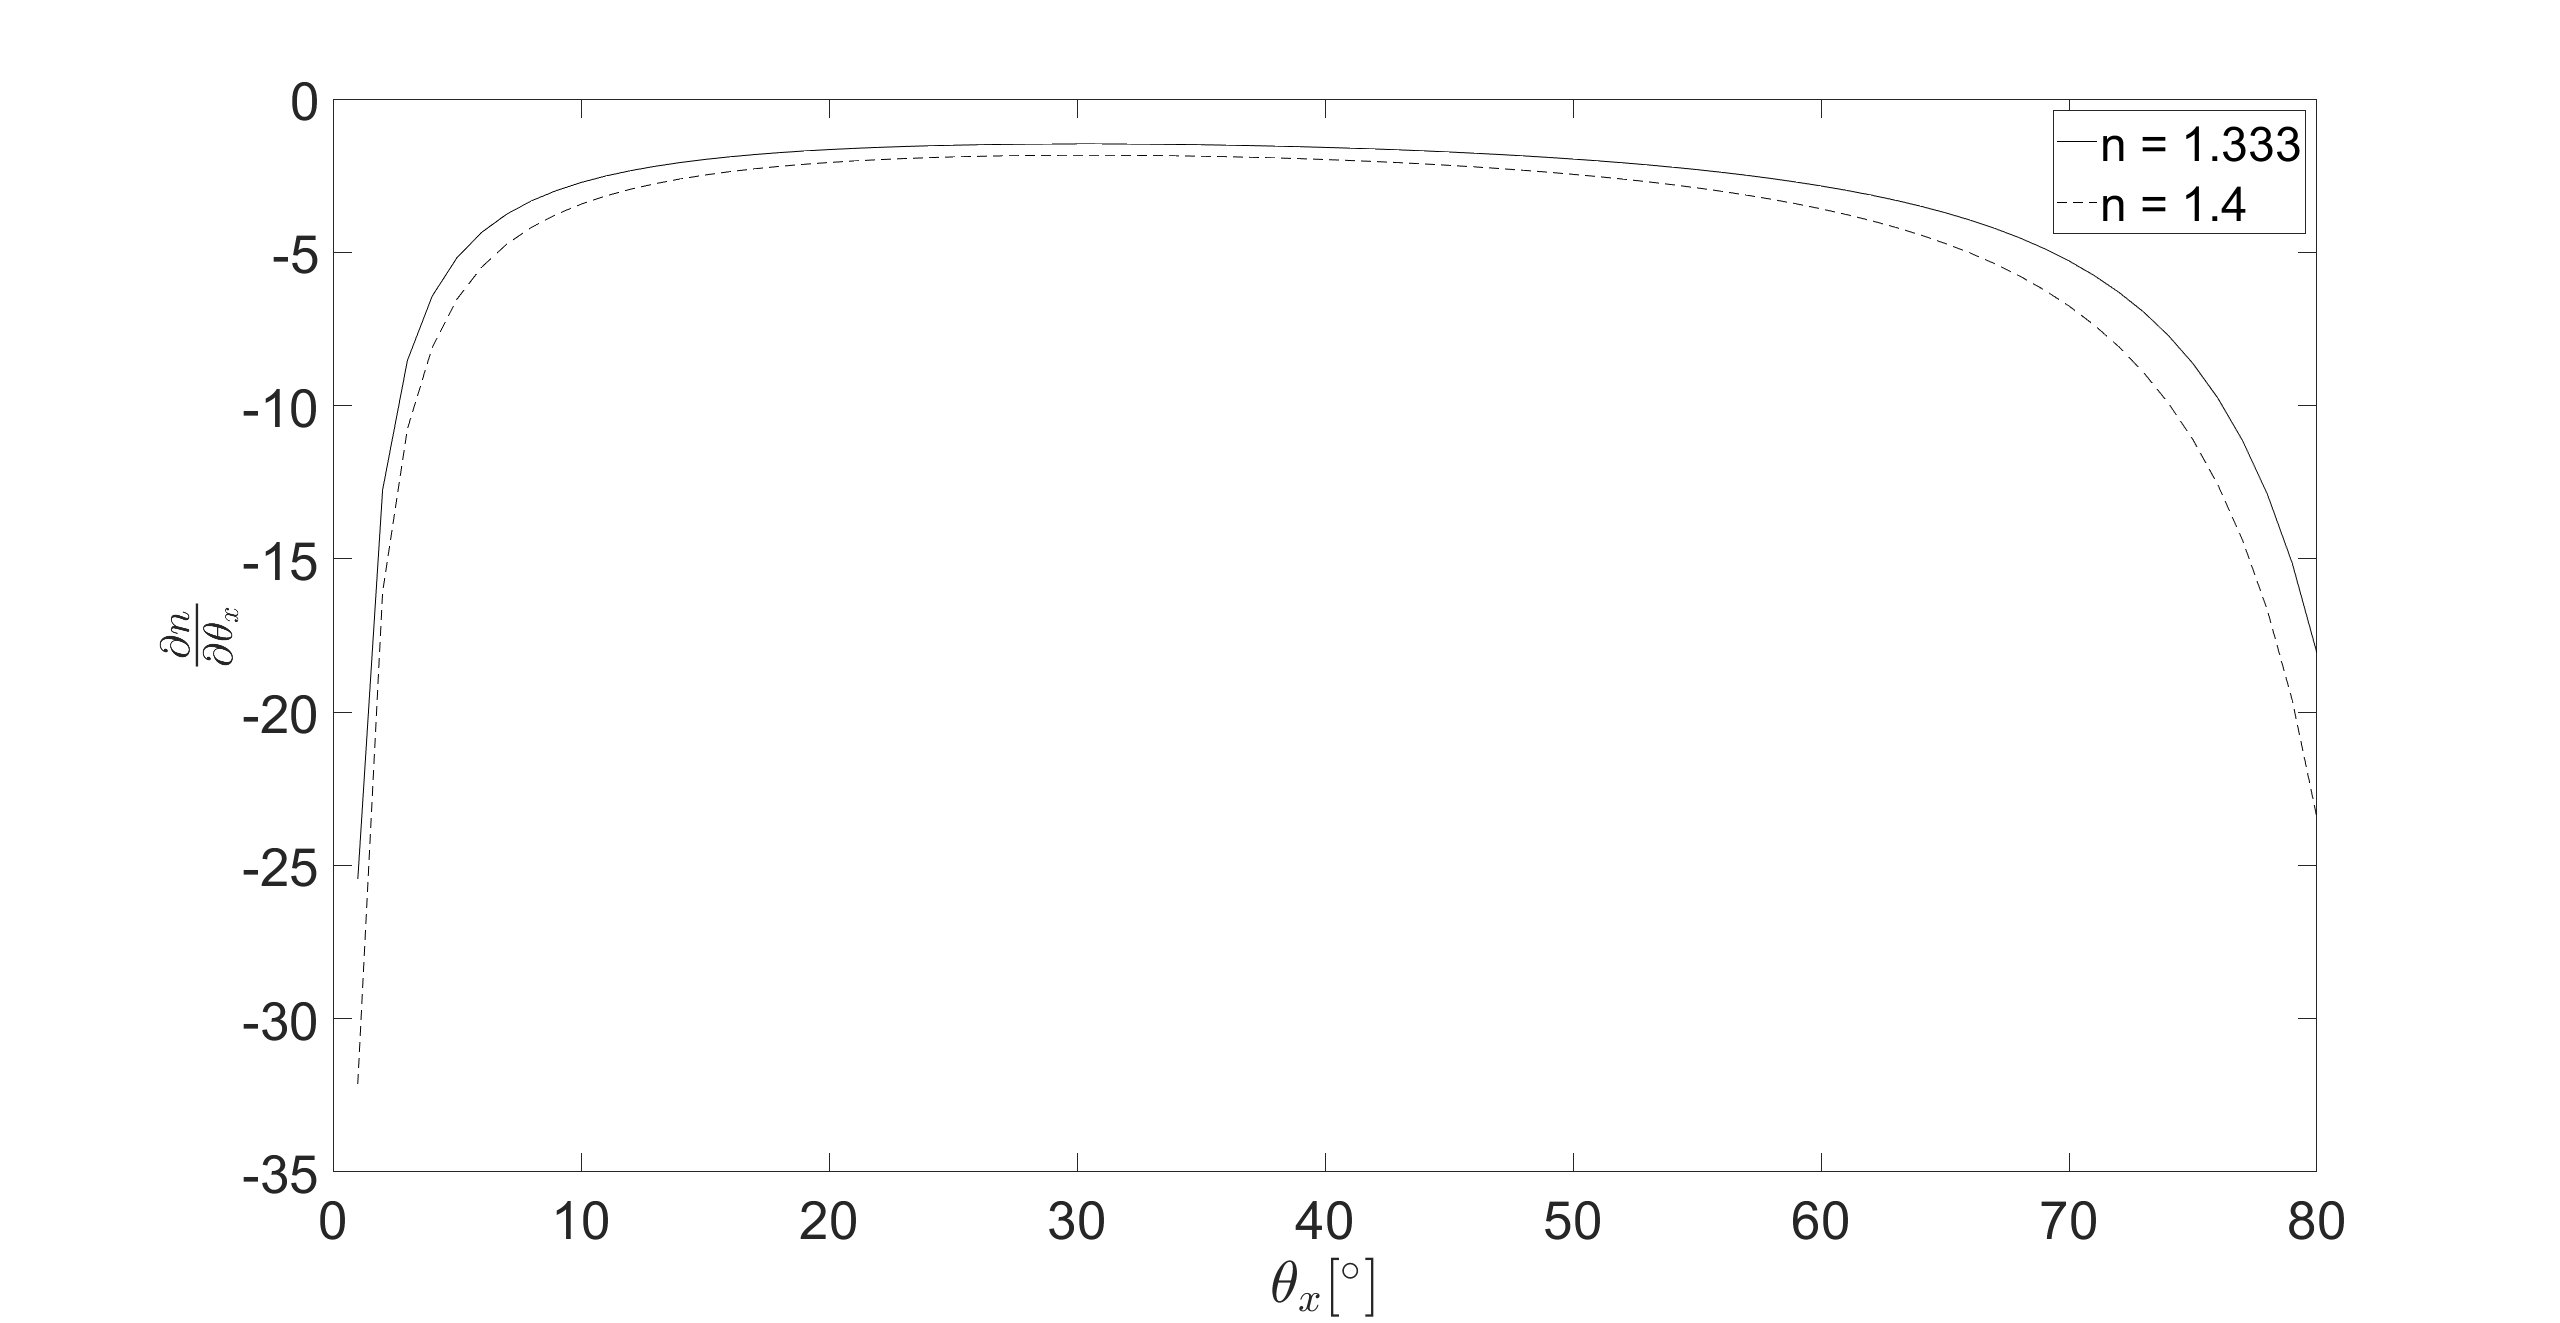
\includegraphics[width=\textwidth, keepaspectratio]{dndt.png}
	\caption{Derivative of $n$ with respect to $\theta_x$ as a function of $\theta_x$.}		
	\label{fig:dndt}
\end{figure}

We want $\Delta x$ to vary with $n$ as much as possible. So, we want $n$ to vary with $\Delta x$ as little as possible.  To find the best angle $\theta_x$ to achieve this, we take the derivative of (\ref{eq:invdexcon2}) with respect to $\Delta x/L_t$ \cite{nemoto1992measurement}. Figure \ref{fig:dndx} show this derivative: $\partial n/\partial (\Delta x/L_t)$ decreases with increasing $\theta_x$. The worst possible angle to measure $\Delta x$ is $0^\circ$.

Since there is also an uncertainty in the angle, we want $n$ to vary with $\theta_x$ as little as possible. Figures \ref{fig:dndt} show this derivative. The magnitude of this derivative $\left|\partial n/\partial \theta_x\right|$ first decreases with increasing $\theta_x$, reaches a minimum, then increases again. The worst possible angles to measure at are $0^\circ$ and $90^\circ$. This minimum is reached at $31^\circ$. Any angle between $15^\circ$ and $60^\circ$ yields approximately the same sensitivity of $n$. 

Viewing at too large an angle (e.g. $70^\circ$) makes it hard to see through the water tank. 
%As an example, we take an index of refraction $n=1.333$, an index of refraction $n_0 = 1$, a tank width $L_t=0.2[m]$ and an angle $\theta_x=30^\circ$. (\ref{eq:dexcon2}) yields a $\Delta x = 0.0345[m]$. From Figure (\ref{fig:dndx}), $\partial n/\partial (\Delta x/L_t) = 2.831$  at $\theta_x = 30^\circ$. Hence an error of $1[mm]$ in $\Delta x$ causes an error of $0.014$ in $n$. From Figure (\ref{fig:dndt}), $\partial n/\partial \theta_x = -1.466$  at $\theta_x = 30^\circ$. Hence an error of $0.1^\circ$ in $\theta_x$ causes an error of $-0.15$ in $n$. 

%To perform accurate measurements we want to determine $n$ with at least 5 significant digits. To achieve this, we place our camera under an angle to minimize the effect of errors in $\Delta x$ and $\theta_x$ on the index of refraction. 

%To reduce

Concluding, Figures \ref{fig:dndx} and \ref{fig:dndt} indicate that the worst angles to measure are close to zero. Angles between $15^\circ$ and $60^\circ$ result in small errors in $n$. 

\clearpage 
\section{Forward Model}
\label{sec:formod}
In this section we build a forward model, relating an index of refraction field $n$, position on the ccd-sensor $\underline{x}$ and parameters $\underline{\alpha}$ to the coordinates $\underline{X}$ where the light rays hits the screen. We seek a model $\underline{X}(n, \underline{\alpha}, \underline{x})$. This is an extension of (\ref{eq:simplex6}). 

In Subsection \ref{subsec:rayequ} we derive the equations governing 3-dimensional ray optics in an inhomogeneous medium. In Subsection \ref{subsec:RayPath} we use these equations to construct the full ray path from the camera through the tank to the screen.

\subsection{Ray Equation} 
\label{subsec:rayequ}
In this section we derive equations describing the paths light rays follow in inhomogeneous media. Inhomogeneous media have a index of refraction $n$ that varies with position.

A curved ray path is a space curve, which we can describe by a parametric representation, $\underline{r}(\sigma) = ( x(\sigma), y(\sigma), z(\sigma))$, where $\sigma$ is an arbitrary parameter. The two most used parameters are (1) the path length long the ray $s$ and (2) the axial position $z$. We denote derivatives with respect to the parameter by dots, so $\dot{\underline{x}}(\sigma) = d\underline{x}(\sigma)/d\sigma$. All parameters are functions of $s$.

The optical length $\mathcal{A}$ of a path $\underline{r}(s)$ taken by a ray of light passing from point $A$ to point $B$ in three-dimensional space is defined by
\begin{equation}
	\label{eq:defAA}
	\mathcal{A} = \int_A^B \! n(\underline{r}(s)) \, \mathrm{d}s,
\end{equation}
where $n(\underline{r})$ is the index of refraction at the spatial point $\underline{r} \in \mathbb{R}^3$. We choose the element of arc length $\mathrm{d}s$ along the ray path $\underline{r}(s)$ through that point as $\mathrm{d}s^2 = \mathrm{d}\underline{r}(s) \cdot \mathrm{d}\underline{r}(s)$, so that $|\dot{\underline{r}}|=1$.

Applying Fermat's principle \cite{holm2011geometric} yields the eikonal equation for ray optics
\begin{equation}
	\label{eq:axialrayequation}
	\frac{\partial n}{\partial \underline{r}} = \frac{d}{ds} \left(n(\underline{r}) \frac{\mathrm{d}\underline{r}}{\mathrm{d} s} \right).
\end{equation}
%Another way to write this ray equation is
%\begin{equation}
	%\label{eq:axialrayequationvector}
	%\nabla n = n \ddot{\underline{r}} + (\nabla n \cdot \dot{\underline{r}}) \dot{\underline{r}}
%\end{equation}
Only two of the component equations are independent, since $|\dot{\underline{r}}| = 1$.
 
To find the equations used in Synthetic Schlieren \cite{weyl1954analysis,dalziel2000whole}, we first derive the axial eikonal equation. Most optical instruments are designed to posses a line of sight (or primary direction of propagation of light) called the optical axis. In Synthetic Schlieren this optical axis coincides with the direction in which the refractive index $n$ does not vary. Choosing a Cartesian coordinate system such that the $z$-axis coincides with this optical axis, expresses the arc-length $\mathrm{d}s$ in terms of the increment along the optical axis, $\mathrm{d}z$. Our parametric description is now in terms of $z$: $\underline{r}(z) = (x(z), y(z), z)$. From our definition of $\mathrm{d}s$
\begin{equation}
	\mathrm{d}s(z) = \sqrt{dx^2(z) + dy^2(z) + dz^2} = \sqrt{1+\dot{x}^2 +\dot{y}^2} d z = \frac{1}{\gamma} d z,
\end{equation}
where $\dot{x} = d x / dz$ and $\dot{y} = dy/dz$ and 
\begin{equation}
	\label{eq:gamma}
	\gamma = \frac{d z}{d s} = \frac{1}{\sqrt{1+\dot{x}^2+\dot{y}^2}} = \cos \theta\leq 1,
\end{equation}
where $\theta$ is the angle the ray makes with the $z$-axis. Using (\ref{eq:gamma}) in (\ref{eq:axialrayequation}) yields the axial eikonal equation %The position of a ray at a fixed value of $z$ is denoted by $[x,y]^T$.
\begin{equation}
	\gamma \frac{d}{dz} \left(n(\underline{r}(z)) \gamma \frac{d \underline{r}(z)}{d z} \right)  = \frac{\partial n(\underline{r}(z))}{\partial \underline{r}}.
\end{equation}
This yields three equations, one for each coordinate direction,
\begin{equation}
	\label{eq:axraycoord}
	\begin{aligned}
		\ddot{x}  &= \frac{1}{\gamma^2} \frac{1}{n} \left(\frac{\partial n}{\partial x} - \dot{x} \frac{\partial n}{\partial z} \right), \\
		\ddot{y} &= \frac{1}{\gamma^2} \frac{1}{n} \left(\frac{\partial n}{\partial y} - \dot{y} \frac{\partial n}{\partial z} \right), \\
		\frac{\partial n}{\partial z} &= \gamma \frac{d}{dz}\left(n  \gamma\right).
	\end{aligned}
\end{equation}	
Indeed, this system of equations shows that only two equations are independent. In Synthetic Schlieren the variation in $n$ in the $z$-direction, the optical axis, is assumed to be zero. Then (\ref{eq:axraycoord}) reduce to
\begin{equation}
	\label{eq:SSeq}
		\ddot{x} = \left(1+\dot{x}^2+\dot{y}^2\right) \frac{1}{n} \frac{\partial n}{\partial x}, \qquad
		\ddot{y} = \left(1+\dot{x}^2+\dot{y}^2\right) \frac{1}{n} \frac{\partial n}{\partial y},
\end{equation}
which are the starting point for the derivation of Synthetic Schlieren in \cite{dalziel2000whole}.  \footnote{The third equation in (\ref{eq:axraycoord}) reduces to $n \gamma = constant$.  To integrate (\ref{eq:SSeq}) we do not need to assume $\dot{x}$ and $\dot{y}$ are small. Experimentally, this means we can apply Synthetic Schlieren even when the angles of the light rays are large. }

In the application presented in this paper, the optical axis does not coincide with the direction in which the refractive index $n$ does not vary. Our parametric description is in the arc-length $s$ and not in $z$.  We cannot solve (\ref{eq:axialrayequation}) analytically, so we solve it numerically. We first write our system of three second-order differential equations as a system of 6 first-order differential equations by introducing a quantity $\underline{T}$ \cite{southwell1982ray} such that (\ref{eq:axialrayequation}) becomes
\begin{equation}
	\label{eq:sys6foeq}
		\frac{d \underline{r}}{d s} = \frac{\underline{T}}{n}, \qquad
		\frac{d \underline{T}}{d s} = \nabla n.
\end{equation}
We apply a Runge–Kutta fourth-order method to solve this system. %Appendix \ref{app:RKS} gives the details.

\subsection{Relating Refractive Index to Ray Path}
\label{subsec:RayPath}
To give our method flexibility and not making assumption on the relative configuration in our experimental setup, we model the light rays as traversing in a three-dimensional space and allow the different elements in the experimental setup to have any alignments.

We place our origin again at the pinhole. The $z$-axis aligns with the optical axis of the camera, i.e. the viewing direction of the camera. All the light entering the camera travels through the pinhole and falls on the ccd-sensor. The $x$- and $y$-axes span a plane through the origin parallel to this ccd-sensor. 

\subsubsection{Plane Definition}
The mathematical definition of a plane is
\begin{equation}
	\label{def:plane}
	\underline{\hat{n}} \cdot (\underline{x}-\underline{x}_0) = 0,
\end{equation}
where $\underline{\hat{n}} = (a,b,c)$ is the unit normal vector of the plane, $\underline{x}$ a random vector within the plane and $\underline{x}_0$ a random point on the plane. Expanding (\ref{def:plane}) yields
\begin{equation}
	a(x-x_0) + b(y-y_0) + c(z-z_0) = 0, 
\end{equation}
or 
\begin{equation}
	\label{eq:planedef2}
	ax+by+cz + d = 0 \qquad \mbox{ with } \qquad d = - a x_0 - b y_0 - c z_0.
\end{equation}
For each of the planes 2 to 6 in Figure \ref{fig:schviepalira}, we can write an equation of the form (\ref{eq:planedef2}). We assume all planes are parallel to each other. Then the parameters $a$, $b$ and $c$ are the same for each plane; only $d$ changes. The distances in the normal direction of each plane are known, e.g. $L_s$, $L_g$, etc. Given the equation describing plane 6, 
\begin{equation}
\label{eq:planedef6}
	a x + b y + c z + d = 0,
\end{equation}
we can compute the equations describing the other planes
\begin{align}
a x + b y + c z + d_i = 0, \qquad  
& d_5 = d + (a+b+c) L_s, \\
& ..., \nonumber \\ 
& d_2 = d + (a+b+c) (L_s+2L_g+L_t), \\
\label{eq:planedef1}
& d_1 = d + (a+b+c) (L_s+2L_g+L_t+L_c) = 0 
\end{align}

\subsubsection{Direction Cosines}
Each pixel in our image corresponds to a physical location on the ccd-sensor with coordinates $\underline{x} = (x,y, -L_f)$, where $L_f$ is the distance from the ccd-sensor to the pinhole in the $z$-direction. We calculate this distance with the thin lens equation
\begin{equation}
 \frac{1}{L_f} + \frac{1}{L_m} = \frac{1}{f},
\end{equation}
where $f$ is the focal length of the camera and $L_m$ is the distance from the pinhole to screen (plane 6) along the $z$-axis. This distance is found from (\ref{eq:planedef6}) for $x=y=0$. Then $d = - c L_m$.

The physical coordinates $x$ and $y$ are obtained from the pixel locations $x_p, y_p$, the pixel locations at $(x,y)=(0,0)$ $x_p^0$ and $y_p^0$ and the physical size of each pixel on the ccd-sensor. Assuming each pixel on the ccd-sensor is square, we call the physical size of each sensor $S^2$. $S$ has units $\mu m/pixel$. The physical coordinates are then found from the pixel locations by
\begin{equation}
	x = S (x_p-x_p^0), \qquad  y = S (y_p-y_p^0).
\end{equation}

Each light ray travels in a straight line from these coordinates $\underline{x}$, through the pinhole, to the experimental setup. We describe each of these light rays with direction cosines: the cosines of the angles between the light ray and the three coordinate axes:
\begin{align}
\label{eq:directioncosines}
	\alpha &= \cos \theta_x = \frac{x}{\sqrt{x^2+y^2+L_f^2}} \nonumber \\
	\beta &= \cos \theta_y = \frac{y}{\sqrt{x^2+y^2+L_f^2}} \\
	\gamma &= \cos \theta_z = \frac{L_f}{\sqrt{x^2+y^2+L_f^2}} \nonumber
\end{align}
At the pinhole, all light rays pass through the origin and have coordinates (0,0,0). Each light ray has direction cosines $(\alpha, \beta, \gamma)$.

\subsubsection{Intersection Light Rays and Planes: Homogeneous medium}
The equation governing light rays in homogeneous media is
\begin{equation}
	\label{eq:linedef}
   \underline{p} = \underline{s} + \underline{I} l,
\end{equation}
where $\underline{s} = (s_x, s_y, s_z)$ is the initial position, $\underline{I} = (\alpha, \beta, \gamma)$ the direction cosines, $p = (p_x, p_y, p_z)$ the final position and $l$ the length traveled along the light ray. %This is the extension of (\ref{eq:simpleline}) in three-dimensions. 

To intersect with a plane, the final position $\underline{p}$ must lie on that plane. Substituting (\ref{eq:planedef2}) into (\ref{eq:linedef}) and solving for $l$ yields 
\begin{equation}
	l = - \frac{d + a s_x + b s_y + c s_z}{a \alpha + b \beta + c \gamma}
\end{equation}
Substituting this $l$ into (\ref{eq:linedef}) yields the location where each light rays intersects with the plane.

\subsubsection{Snell's Law}
To find the angle of incidence, $\theta_I$, between the incoming light ray and the plane, we compute
\begin{equation}
	\cos \theta_I = \underline{\hat{n}} \cdot \underline{I}.
\end{equation}
We apply Snell's law (\ref{eq:snellslaw}) to find the angle of refraction, $\theta_T$. The index of refraction of the medium through which the incoming ray travels is $n_I$, the index of refraction of the medium through wich the outgoing ray travels is $n_T$. To find the direction cosines of the outgoing ray, $\underline{T}$, we calculate 
\begin{align}
	S &= \sign \cos \theta_I, \\
	\sin \theta_T &= \frac{n_I}{n_T} \sqrt{1-\cos^2 \theta_I}, \\
	\cos \theta_T &= \sqrt{1-\left(\frac{n_I}{n_T}\right)^2(1-\cos^2 \theta_I)} \\
	\underline{T} &= \frac{n_I}{n_T} \underline{I} + \left(\frac{n_I}{n_T} \cos \theta_I - S \cos\theta_T\right)\underline{\hat{n}},	
\end{align}
where $S$, the sign of $\cos\theta_I$ ensures we stay in the right quadrant.

\subsection{Displacements}
Previous subsections combine to give the forward model: $\underline{X}(n,\underline{\alpha}, \underline{x})$. Given an index of refraction field $n$, parameters $\underline{\alpha}$ and coordinates $\underline{x} = (x,y)$, we can calculate the location on the screen where the light rays end up. $\underline{\alpha}$ are the parameters that define the planes $a$, $b$, $c$ and $L_m$. We use $L_m$ instead of $d$ since we want our parameters to be (linearly) independent. Also, $L_m$ has a clear geometric meaning.

We take our forward model twice, once for a known index of refraction (typically constant) $n_0$ and once for an unknown index of refraction field $n$. The light rays originating from the same location on the screen end up on different locations on the ccd sensor:
\begin{equation}
\label{eq:ForwardModel}
	 \underline{X}(n, \underline{\alpha}, \underline{x}+\underline{\Delta x}) - \underline{X}(n_0, \underline{\alpha}, \underline{x}) = 0, \qquad \underline{X} = (X, Y, Z).
\end{equation}
This equation holds for each measured displacement $\underline{\Delta x} = (\Delta x, \Delta y)$. From (\ref{eq:directioncosines}) we see that light rays with different locations on the ccd-sensor have different angles with which they leave the camera. Due to the different index of refraction in the tank, they do end up in the same location on the screen.

\section{Calibration}
\label{sec:cal}
In our forward model in Section \ref{subsec:RayPath}, we have used the parameters describing a plane $a$, $b$ and $c$ and $L_m$. However, when setting up a new experiment, these are not known. To obtain these, we perform a calibration step. This calibration determines the parameters very precisely and gives us a lot of experimental freedom. For example, we do not have to align the camera, or even measure the position of the camera relative to the water tank. We use calibration for this.

The calibration consists of performing one extra measurement (two in total): we take a reference image, the tank without water (filled with air) and a deformed image, the tank filled with water with a known index of refraction. The easiest is water without any salts. Performing DIC yields us the displacements $\Delta \underline{x}$. This allows us to determine the parameters $\underline{\alpha}.$

In our simple model, this calibration is the equivalent of (\ref{eq:dexcon2}). We know $n$, $n_0$ and $\Delta x$ and we want to determine $\alpha$ (from $\theta_x = \alpha+\phi_x$).

Looking at our Forward Model (\ref{eq:ForwardModel}), we know
\begin{enumerate}
	\item $n=n_0$ and $n=n_1$, the index of refraction of reference image (filled with air) and the deformed image (filled with water); 
	\item $\underline{x}$, the coordinates on our ccd-sensor; 
	\item $\underline{\Delta x}$, the measured displacement (after DIC). 
\end{enumerate}
The unknowns are the parameters $\underline{\alpha} = (a, b, c, L_m)$. Since we have only four parameters to estimate and many measurements (each grid point yields a separate equation), we have an over-determined system. We use a least-squares approach to find those $\underline{\alpha}$ that minimize the sum of squares of the residuals. The forward model depends nonlinearly on the parameters $\alpha$ and the measurements $\underline{\Delta x}$. For each measurement $\underline{\Delta x}$ we have a measure of reliability, the correlation coefficient, which we use as a weight $w$ in the least squares procedure
\begin{equation}
\label{eq:calmin} 
\min_{\underline{\alpha}}  S = \min_{\underline{\alpha}} \sum_i w_i \left(X_{j}(n_1, \underline{\alpha}, \underline{x}_i+\underline{\Delta x}_i) - X_{j}(n_0, \underline{\alpha}, \underline{x}_i)\right)^2, 
\end{equation}
with constraints (1) $L_c > 0$ and (2) $L_m \geq L_c + 2 L_g + L_t + L_s$, the experimental setup is in front of the camera; (3) $c < 0$, the unit normal vector of the planes points in the negative $z$-axis. Combining these constraints implies $d>0$. The sum is over all measured displacements. The weights $w_i$ are $0$ when $CC < 0.8$ and $1$ otherwise. We use only the displacements in the $x$-direction, since that is the direction with the largest angles and thus largest signal.

The distance $L_c$ between the camera and the front of water tank (plane 2) along the $\underline{\hat{n}}$ direction is obtained from the total distance $d$ between the camera and the screen along the $z$-direction and the distances $L_g, L_t$ and $L_s$. This ensures internal consistency in our model. We obtain $L_c$ from (\ref{eq:planedef1}).

To find the best way to solve (\ref{eq:calmin}), Figures \ref{fig:Sab} to \ref{fig:ScLm} show $S$ as a function of $\underline{\alpha}$ for a typical experiment. For each figure, we have fixed two parameters of $\underline{\alpha}$ and varied the other two. The blue lines indicate the constraint $L_c >0$ and the red lines indicate the constraint $L_m \geq L_c + 2 L_g + L_t + L_s$. The black cross indicates the global minimum in the allowable region.

All figures show very nice behavior of $S$. Figures \ref{fig:Sab}, \ref{fig:Sac} and \ref{fig:SbLm} show one clear minimum in the allowed region. Figures \ref{fig:Sac}, \ref{fig:SaLm} and \ref{fig:ScLm} show one clear valley in the allowed region. 

It seems that when we choose an initial condition that falls in the permissible regions and use a gradient-based optimization scheme we will end up in the minimum. %Only one minimum exists in each of the permissible regions. 

\begin{figure}[htbp]
		\centering 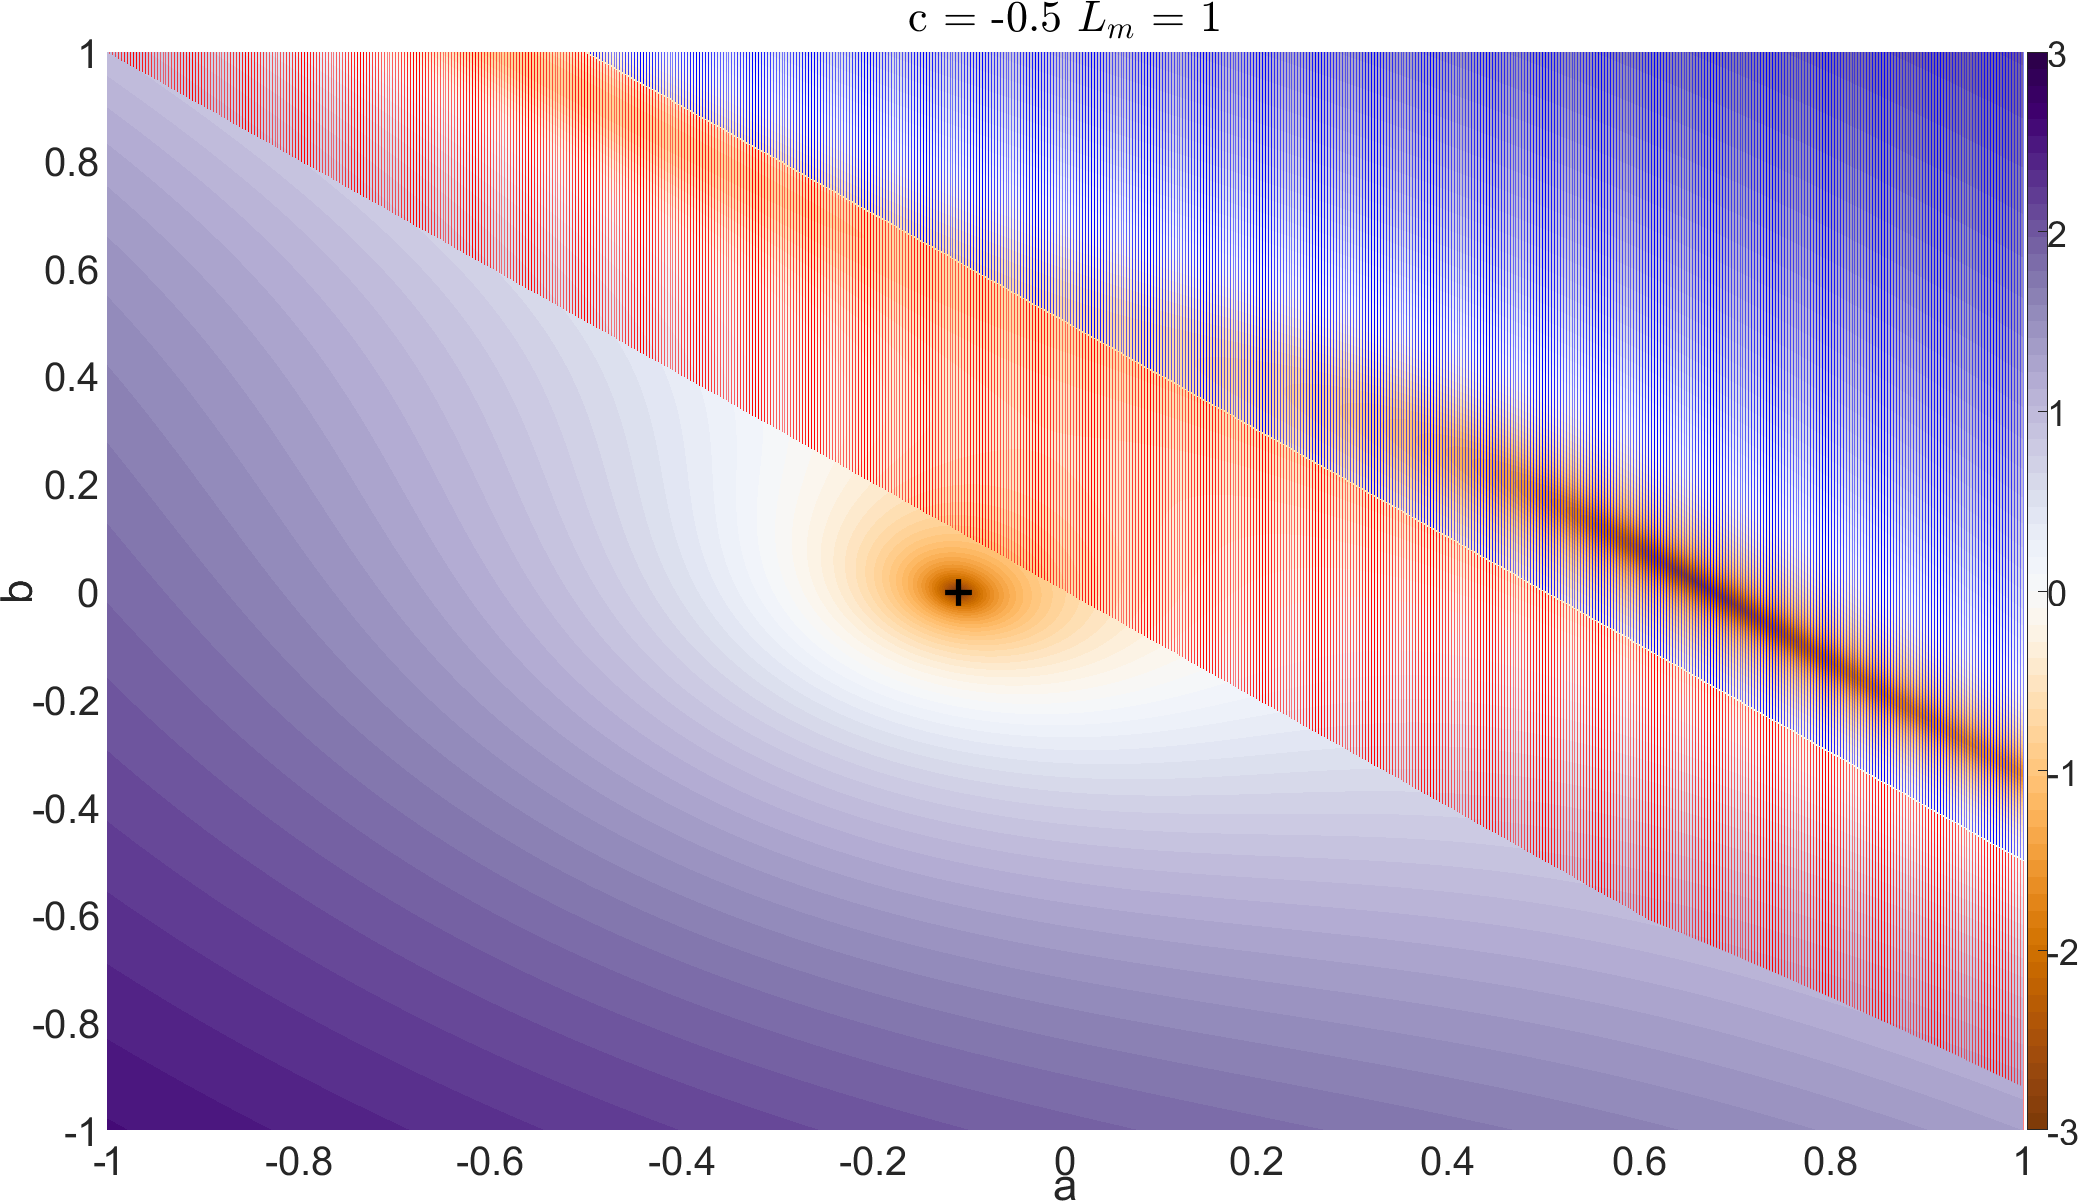
\includegraphics[width = \textwidth]{leastsquaresab.png}
		\caption{$\log_{10}S(a,b)$}\label{fig:Sab}
\end{figure}
\begin{figure}[htbp]
		\centering 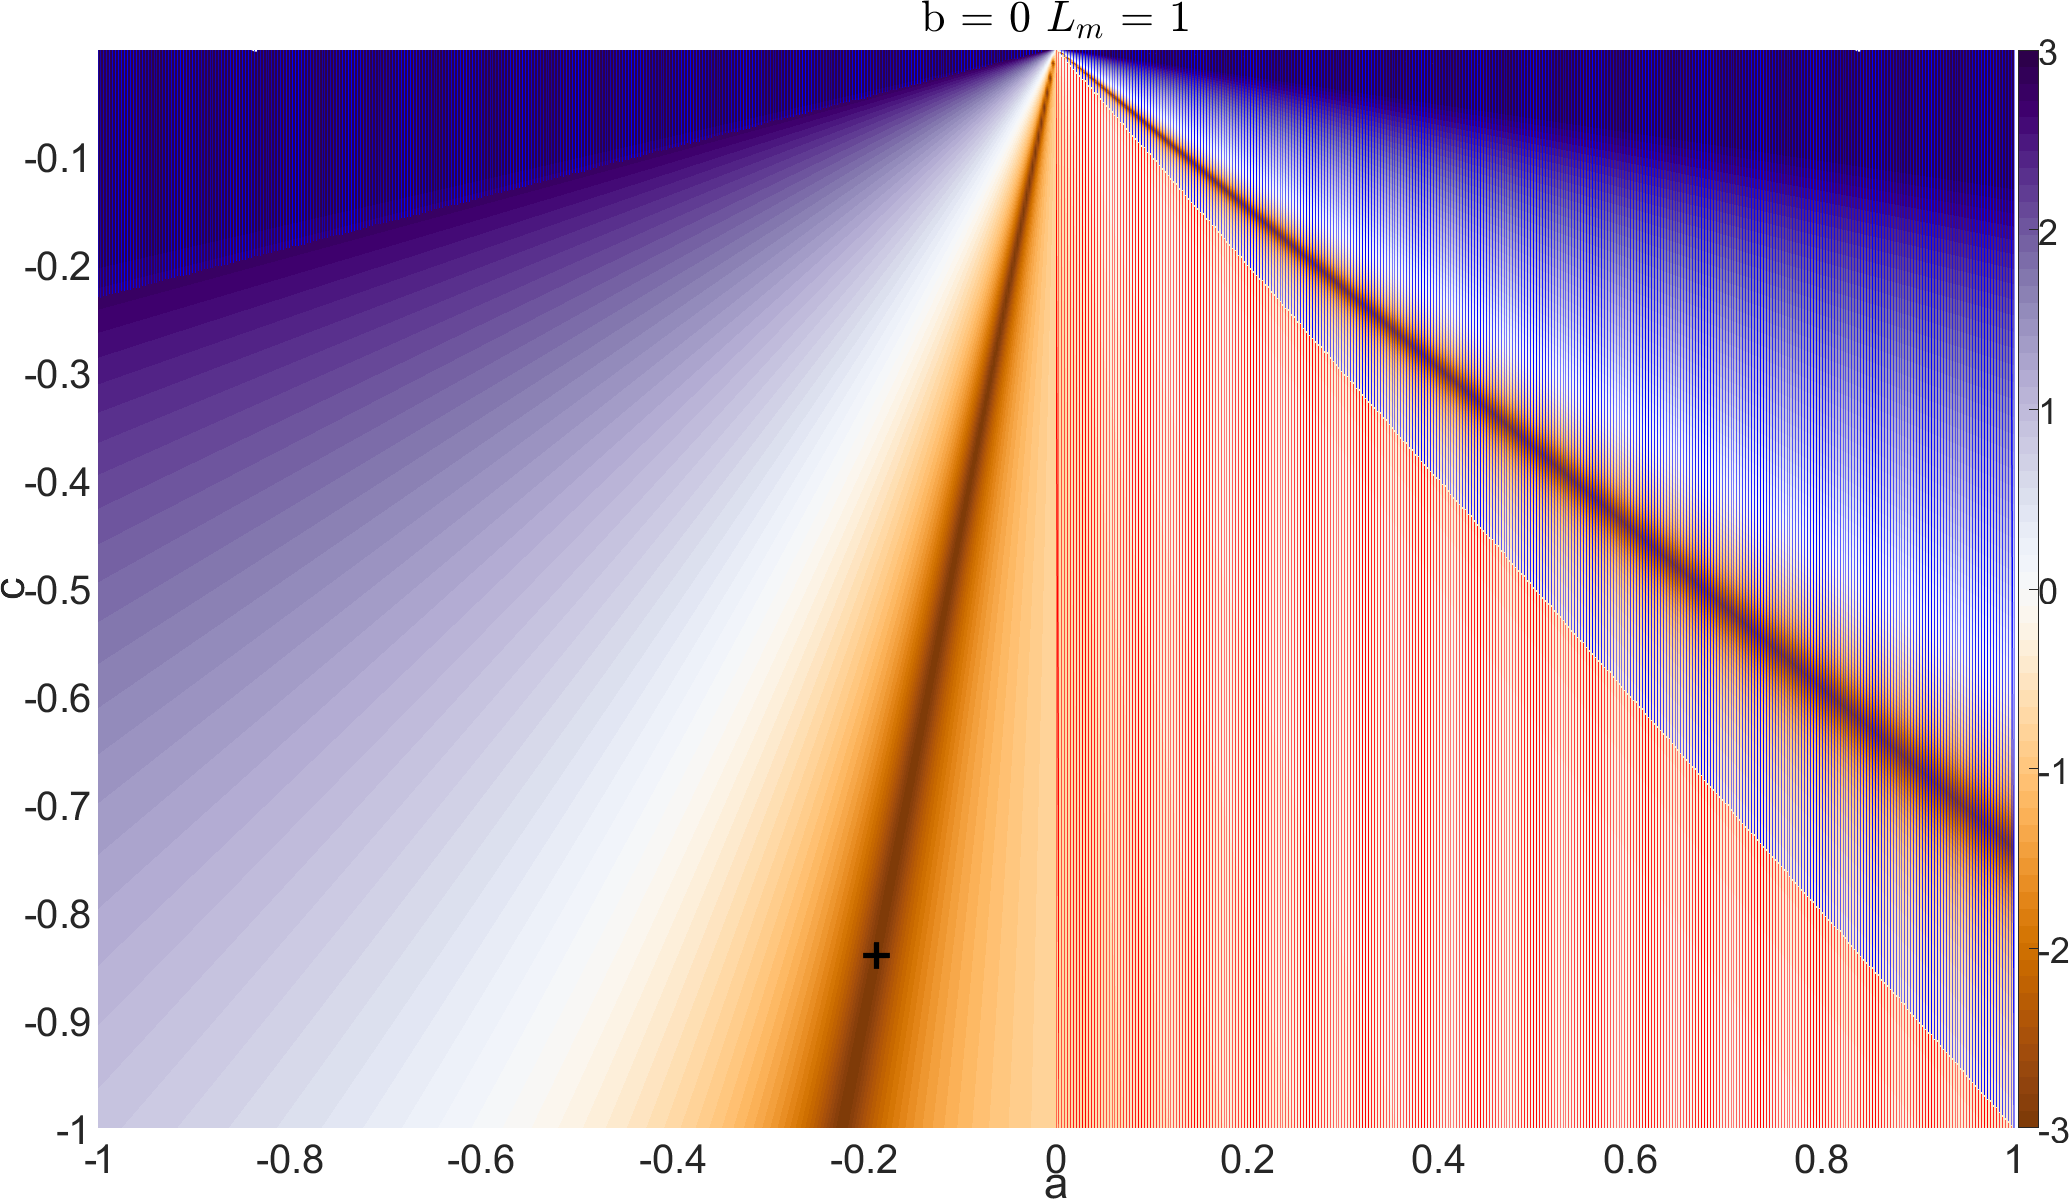
\includegraphics[width = \textwidth]{leastsquaresac.png}
		\caption{$\log_{10}S(a,c)$}\label{fig:Sac}
\end{figure}
\begin{figure}[htbp]
		\centering 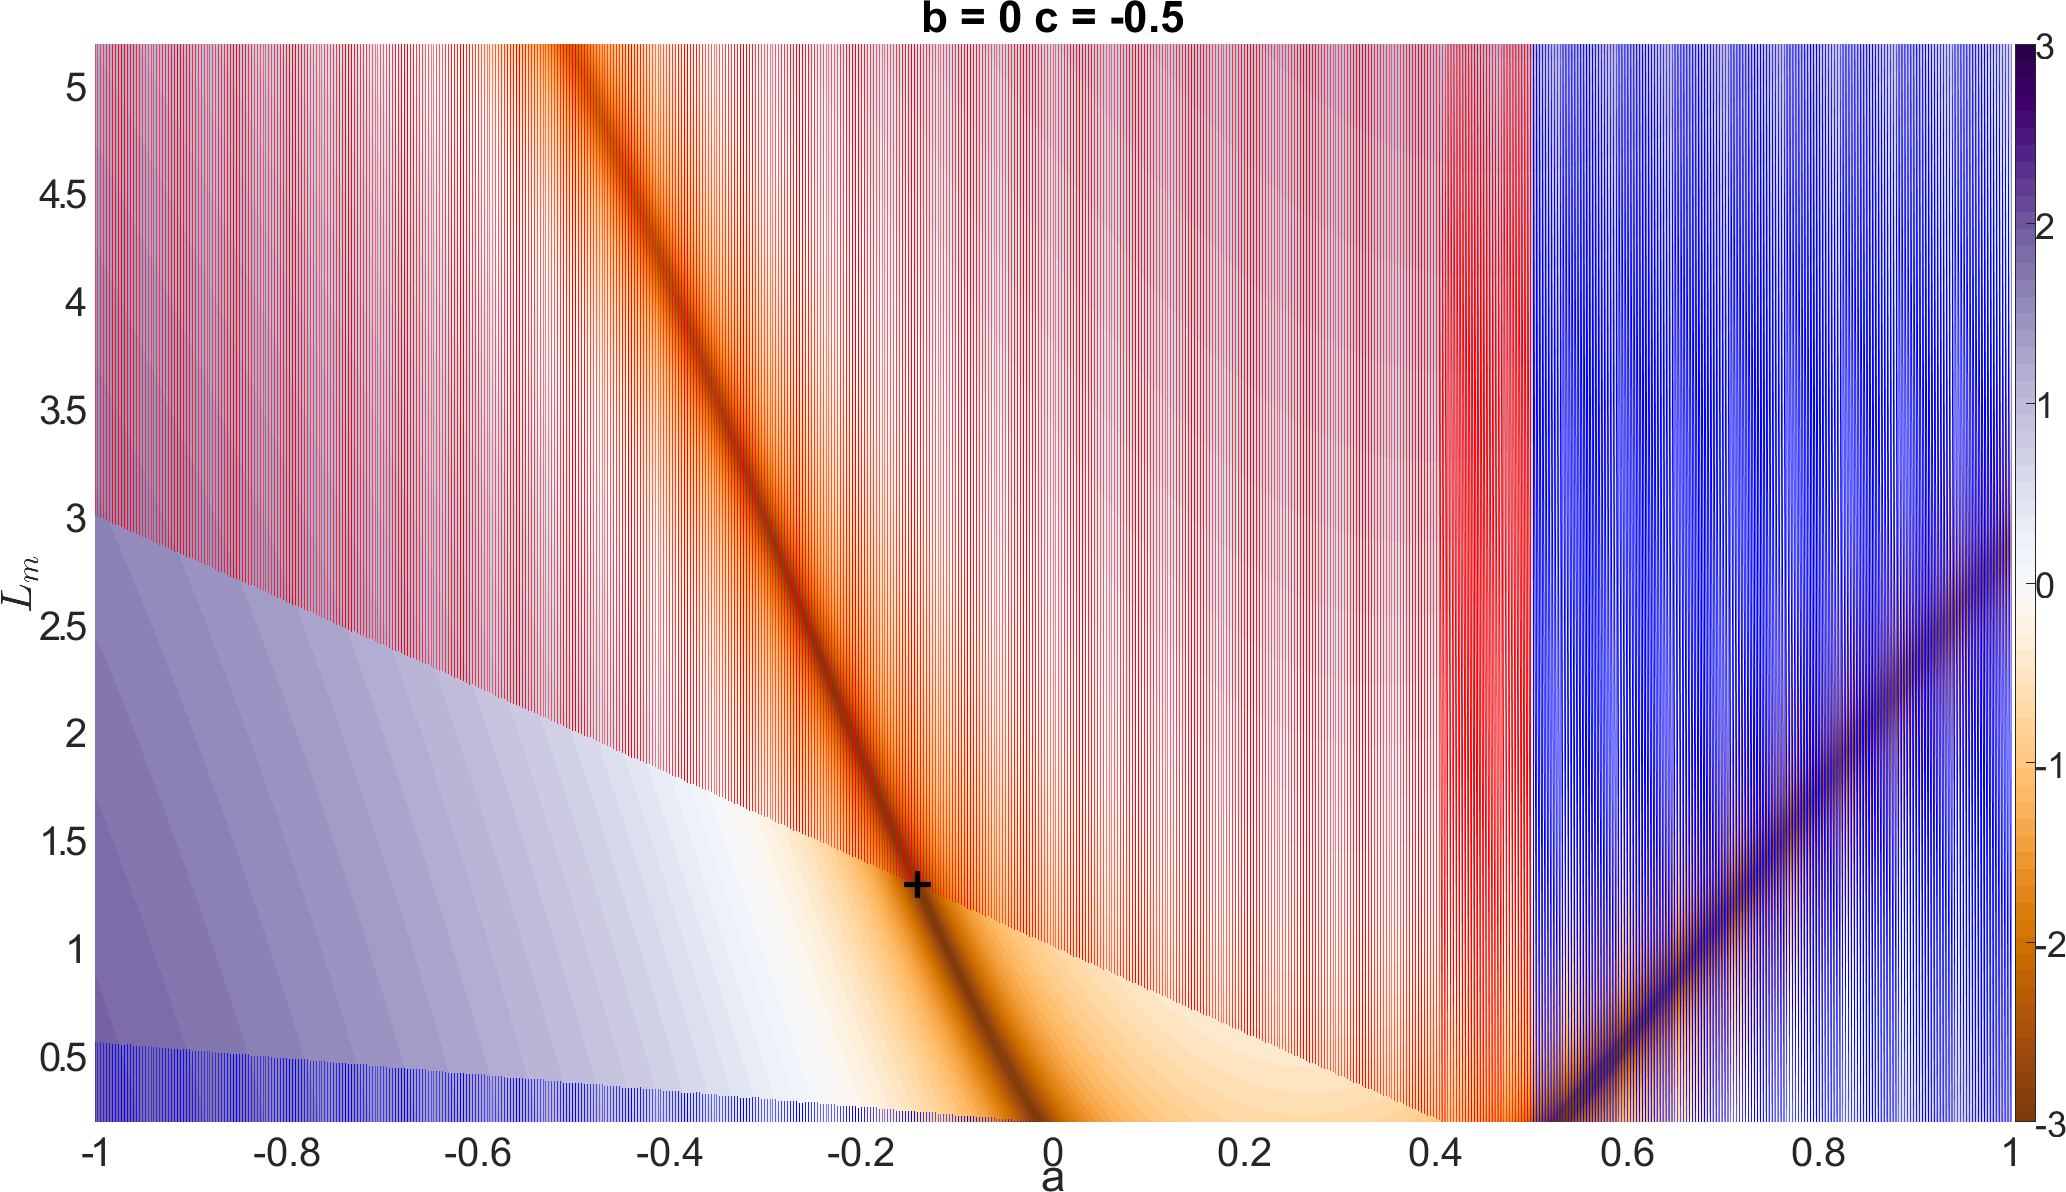
\includegraphics[width = \textwidth]{leastsquaresad.png}
		\caption{$\log_{10}S(a,d)$}\label{fig:SaLm}
\end{figure}
\begin{figure}[htbp]
		\centering 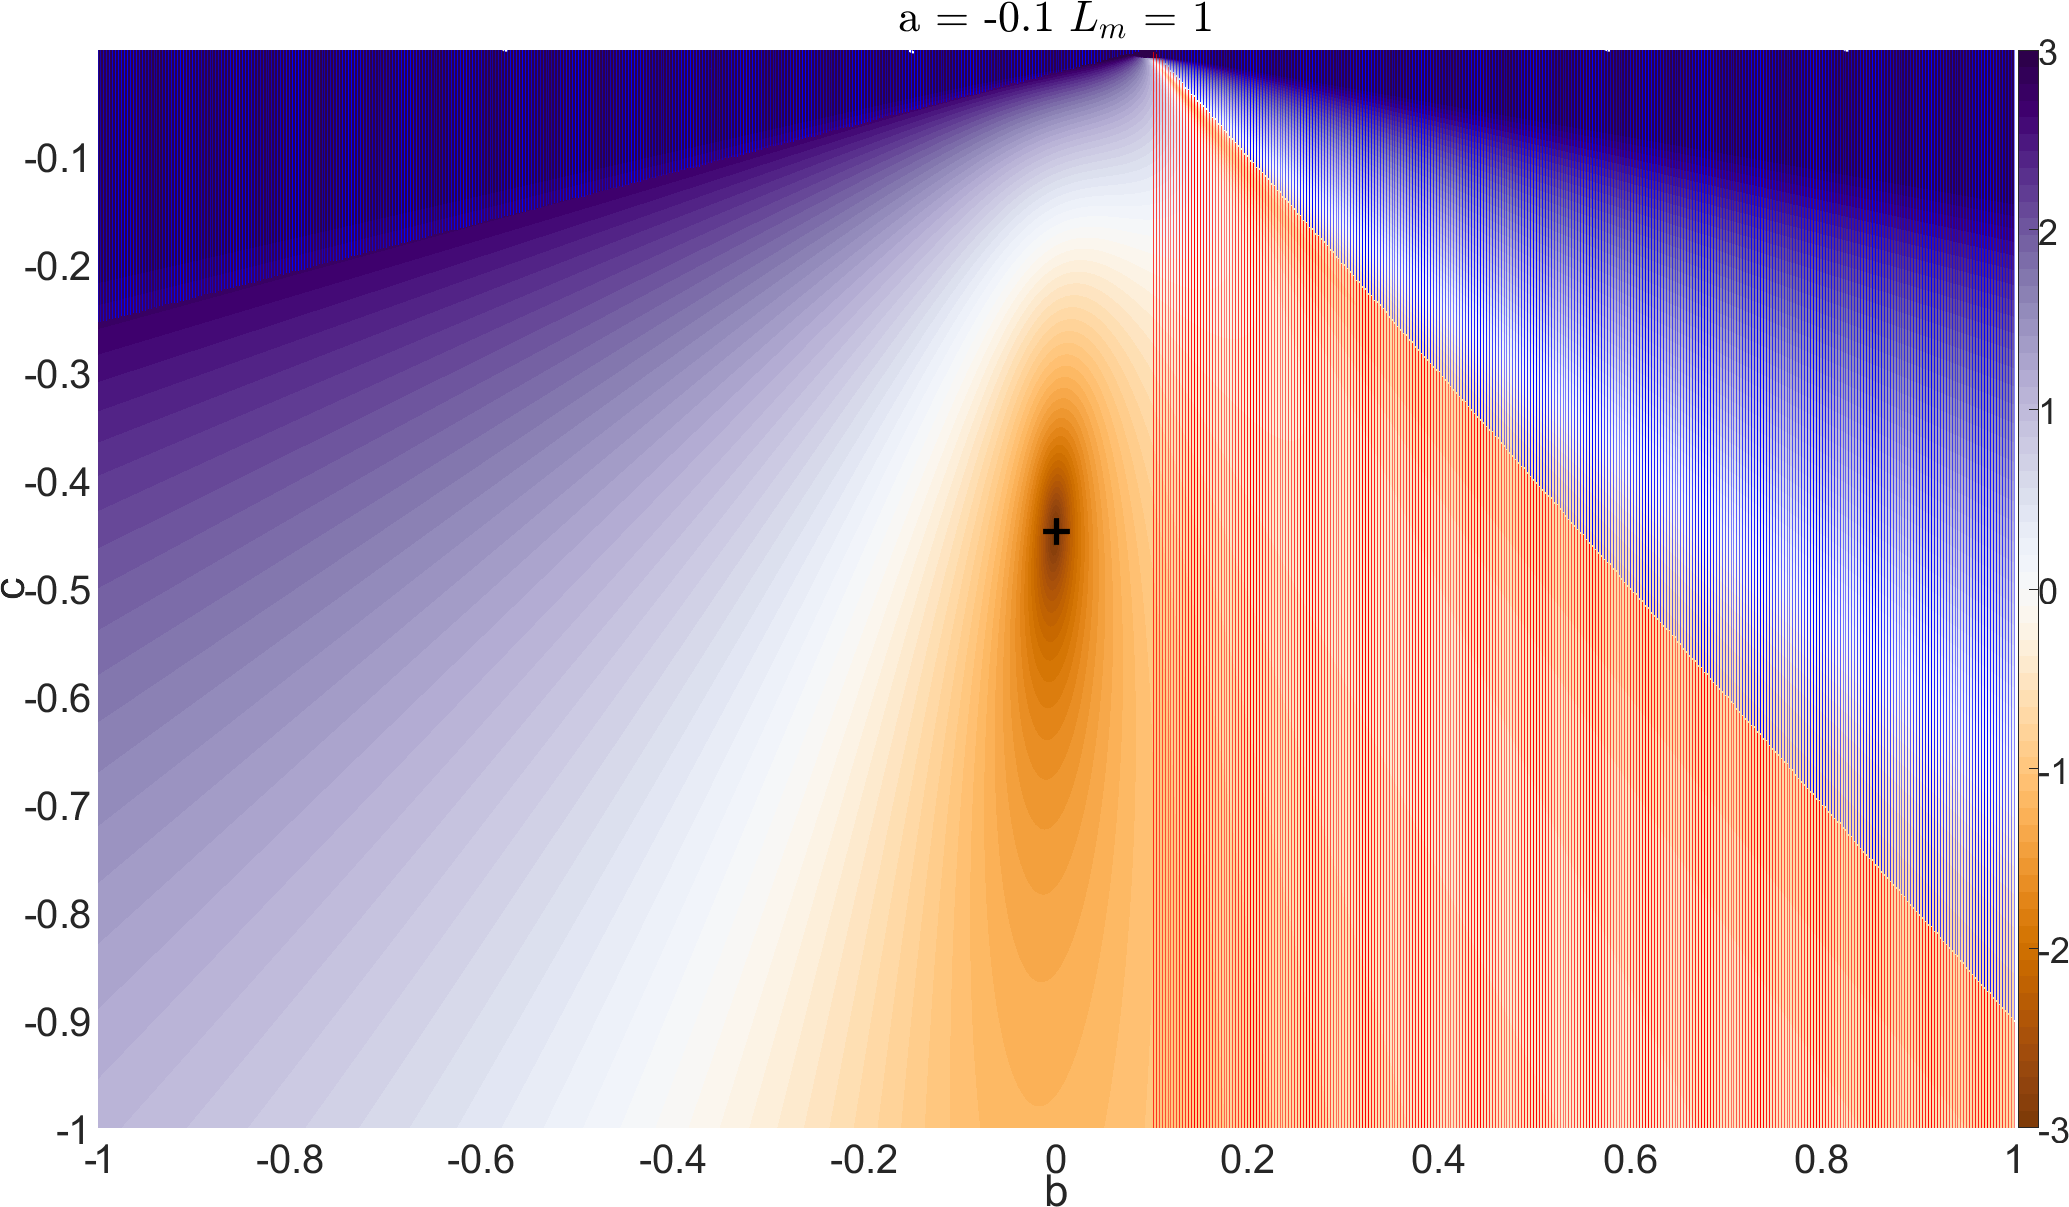
\includegraphics[width = \textwidth]{leastsquaresbc.png}
		\caption{$\log_{10}S(b,c)$}\label{fig:Sbc}
\end{figure}
\begin{figure}[htbp]
		\centering 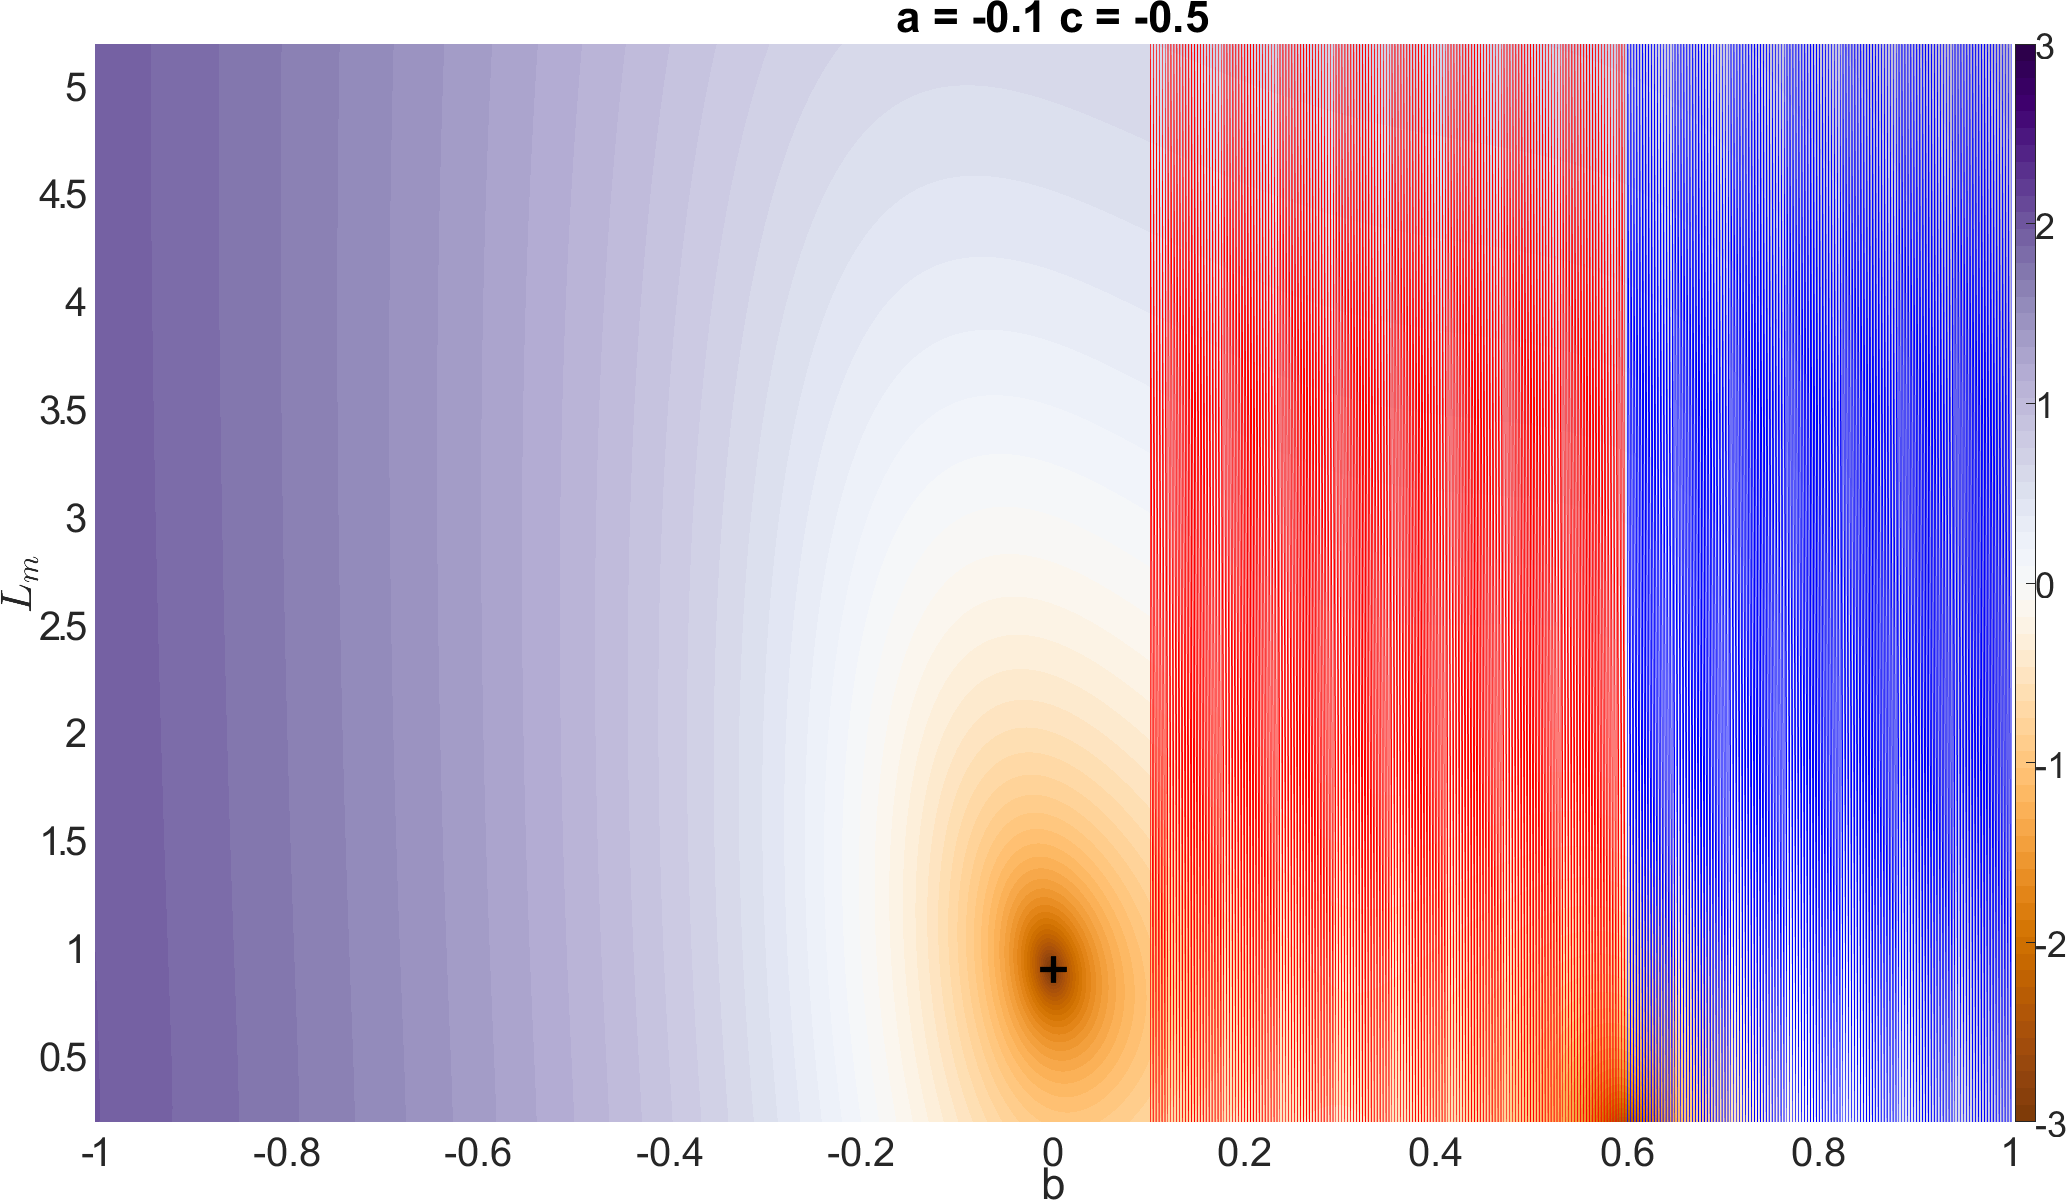
\includegraphics[width = \textwidth]{leastsquaresbd.png}
		\caption{$\log_{10}S(b,d)$}\label{fig:SbLm}
\end{figure}
\begin{figure}[htbp]
		\centering 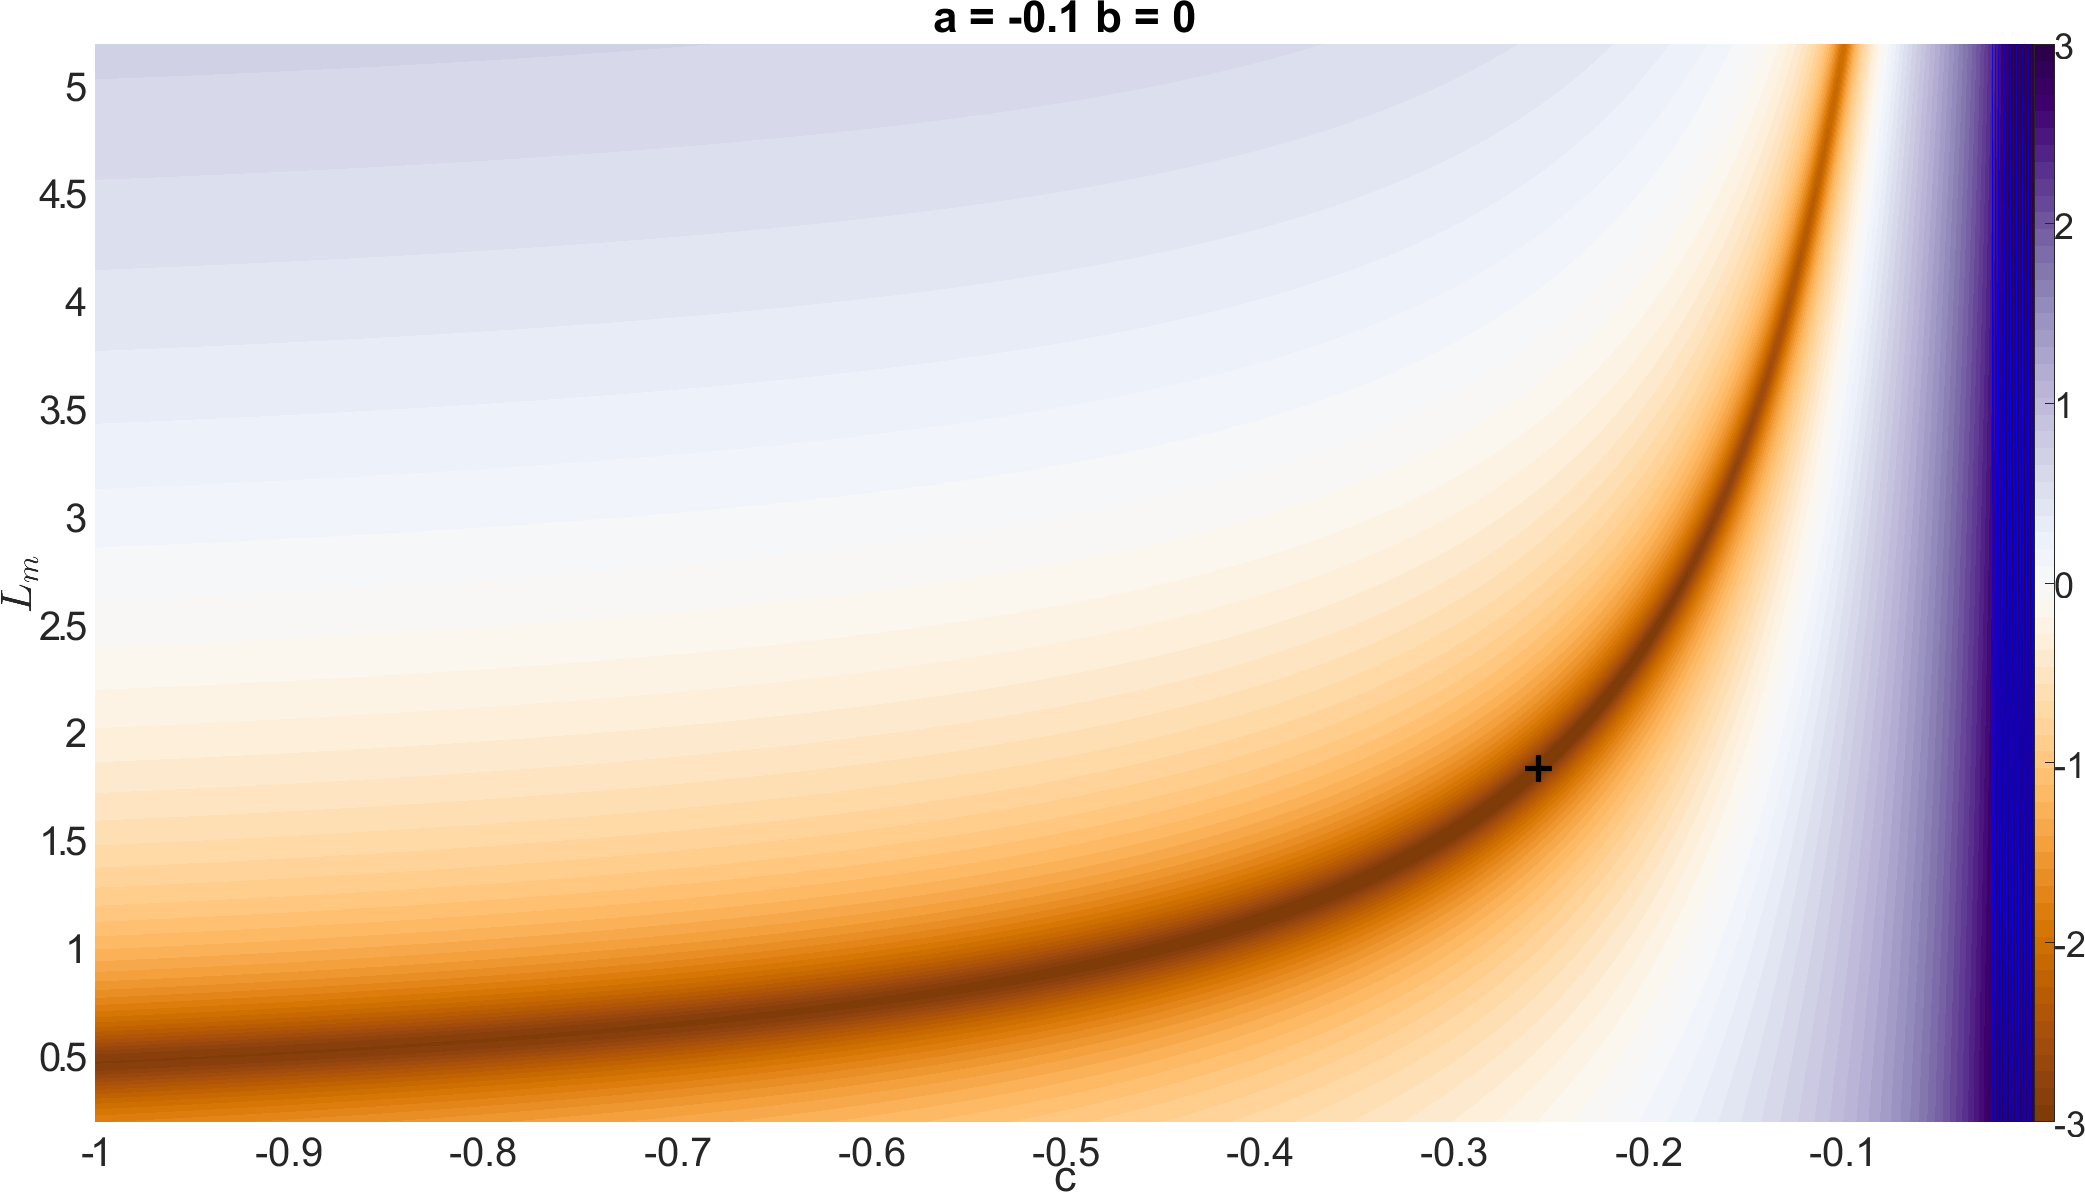
\includegraphics[width = \textwidth]{leastsquarescd.png}
		\caption{$\log_{10}S(c,d)$}\label{fig:ScLm}
\end{figure}

\clearpage

\section{Digital Image Correlation}
\label{sec:DIC}
Digital Image Correlation (DIC) is a well known technique \cite{sutton2009image} to obtain deformation maps from images. We use second-order shape functions \cite{lu2000deformation} to handle large nonlinear deformations. To attain sub-pixel accuracy we interpolate our images with B-splines \cite{thevenaz2000interpolation, unser1999splines, thevenaz2000image}. To obtain the deformations we optimize a Correlation Coefficient, the ZNSSD \cite{sutton2009image}. We solve this nonlinear least-squares problem  by (1) providing an initial guess and (2) solving an iterative scheme. As an initial guess we perform Template Matching \cite{lewis1995industrial,opencv_library} on a limited set of points to obtain rigid deformations with pixel accuracy. After applying DIC to obtain sub-pixel deformations, we use reliability guided DIC \cite{pan2012incremental} with a propagation function \cite{zhou2012propagation} to determine the initial guesses. As iterative scheme we use the Levenberg–Marquardt algorithm. 


\begin{table}[htbp]
\caption{Digital Image Correlation }
\label{tab:esterrmagn}
\centering
\begin{tabular}{ll}
Noise & \\
Subset Size & \\
Grid Size 	& \\
Measurements Points & \\
Total Number of Images & \\
Number of Averaged Images & \\
Displacements & \\
\qquad Spatial Resolution & x pixels, x mm \\
\qquad Resolution & x pixels (x mm) \\
Index of Refraction & \\
\qquad Smoothing Method & \\
\qquad Resolution & x \\
\end{tabular}
\end{table}

Table \ref{tab:esterrmagn} shows the typical DIC parameters used in our experiments. Additionally, the accuracy of the obtained displacements is given.

\section{Experimental}
\label{sec:exp}
Best practices to get good quality images

random dot pattern -> grey -> histogram no over/under saturation 

\section{Inverse Model}
\label{sec:invmod}
Looking at our Forward Model (\ref{eq:ForwardModel}), we know
\begin{enumerate}
	\item $\underline{\alpha}$, the parameters of our experimental setup (after calibration), 
	\item $\underline{x}$, the coordinates on our ccd-sensor, 
	\item $\underline{\Delta x}$, the measured displacement (after DIC), 
	\item $n_0$, the index of refraction of the reference state.
\end{enumerate}
The unknown is the index of refraction field $n$. Unlike the simple model (\ref{eq:invdexcon2}), we cannot invert the forward model to obtain an expression for the index of refraction $n$. We treat the problem of finding $n$ as an optimization problem:
\begin{equation}
\label{eq:nmin} 
\min_{n_i}  S = \min_{n_i} (X_{j}(n, \underline{\alpha}, \underline{x}_i+\underline{\Delta x}_i) - X_{j}(n_0, \underline{\alpha}, \underline{x}_i))^2, 
\end{equation}
with constraints $1.333 \leq n_i \leq 1.4$. For each measurement $\underline{\Delta x}_i$ we solve (\ref{eq:nmin}) to find $n_i$.

Since we are working with liquids we use the Lorentz-Lorenz equation to relate the index of refraction $n$ to the density $\rho$ \cite{lorentz1916theory, tan2015dependence},
\begin{equation}
 	\frac{n^2-1}{n^2+2} \frac{1}{\rho} = \mbox{ constant}.
\end{equation}

\section{Results}
In this section we show three applications of the new method: (1) A static two-layer fluid with large nonlinear deformations, (2) A static stratified fluid and (3) a dynamic fluid/flow? with wave attractor.

In the first application, in \ref{fig:0side}, we want to measure the background density of a two-layer fluid system. We filled the bottom half of a tank with Wadden Sea water (with an index of refraction of 1.338) \footnote{Measured by a refractometer: The Atago Urine Specific Gravity Refractometer with a refractive index range of 1.333-1.356 and a resolution of 0.0005.} and the upper half of the tank with tap water (with an index of refraction of 1.333). We kept the interface between the two layers sharp by filling the upper half of the tank through a sponge. The observed deformations of the dot pattern through this interface are large. Through the use of the second-order shape functions in the DIC procedure, we can still determine these deformations. Figure \ref{fig:ndeformed0side} shows the index of refraction field $n$. The expected theoretical density profile is an error function. We see this in Figure \ref{fig:ndeformed0side}.

\begin{figure}[htbp]
\begin{subfigure}{.5\linewidth}
%		\centering \includegraphics[width = \textwidth]{}
		\subcaption{Reference Image: Filled with air}\label{fig:air0side}
\end{subfigure}%
\begin{subfigure}{.5\linewidth}
%	\centering \includegraphics[width = \textwidth]{}
	\subcaption{Calibration Image Image: Filled with water with known $n$}\label{fig:fresh0side}
\end{subfigure}\\
\begin{subfigure}{.5\linewidth}
%		\centering \includegraphics[width = \textwidth]{}
		\subcaption{Deformed Image: Filled with salt water with unknown $n$-field }\label{fig:twolayer0side}
\end{subfigure}%
\begin{subfigure}{.5\linewidth}
%	\centering \includegraphics[width = \textwidth]{}
	\subcaption{Index of Refraction $n$ for Calibration Image}\label{fig:ncalibration0side}
\end{subfigure}\\
\begin{subfigure}{.5\linewidth}
%		\centering \includegraphics[width = \textwidth]{}
		\subcaption{$\Delta x$ from DIC}\label{fig:dx0side}
\end{subfigure}%
\begin{subfigure}{.5\linewidth}
%	\centering \includegraphics[width = \textwidth]{}
		\subcaption{$\Delta y$ from DIC}\label{fig:dy0side}
\end{subfigure}\\
\begin{subfigure}{.5\linewidth}
%		\centering \includegraphics[width = \textwidth]{}
		\subcaption{Index of Refraction $n$ for Deformed Image}\label{fig:ndeformed0side}
\end{subfigure}%
\begin{subfigure}{.5\linewidth}
%	\centering \includegraphics[width = \textwidth]{}
		\subcaption{Correlation Coefficient from DIC}\label{fig:C0side}
\end{subfigure} \\
\begin{subfigure}{.5\linewidth}
%	\centering \includegraphics[width = \textwidth]{}
		\subcaption{$n$ profiles for Calibration and Deformed Images}\label{fig:nprofiles0side}
\end{subfigure}
\caption{The procedure for obtaining the index of refraction field $n$. We obtain three images: one Reference Image (\ref{fig:air0side}) filled with air, one Calibration Image (\ref{fig:fresh0side}) filled with water without salts and one Deformed Image (\ref{fig:twolayer0side}) filled with water with an unknown $n$-field. Applying DIC between the Reference Image and the Correlation image, we find the displacements $D=(\Delta x, \Delta y)$. Using these displacements $D$ in (\ref{eq:calmin}), we obtain the parameters $\underline{\alpha}$. After calibration, the resulting $n$-field is uniform (\ref{fig:ncalibration0side}). Applying DIC between the Reference Image and the Deformed Image, we find the displacements $\Delta x$ (\ref{fig:dx0side}) and $\Delta y$ (\ref{fig:dy0side}) with corresponding Correlation Coefficient (\ref{fig:C0side}).  Using these displacements in (\ref{eq:nmin}), we obtain the unknown index of refraction field $n$ (\ref{fig:ndeformed0side}). Horizontally averaging the index of refraction fields $n$ yields the profiles in \ref{fig:nprofiles0side}.}
\label{fig:0side}
\end{figure}

\begin{table}[htbp]
\caption{Angles $\beta$ of internal wave beams as a function of the forcing frequency $\omega$. These were determined by a Synthetic Schlieren setup.}
\label{tab:SSintwav}
\centering
\begin{tabular}{llllll}
$\omega$ & 1 & 1 & 1 & 1 & 1  \\
$\beta$  & 1 & 1 & 1 & 1 & 1
\end{tabular}
\end{table}

In the second application, in Reference, we want to measure the background density of a continuously stratified fluid. We filled a tank through the double bucket method. After taking a Reference Image, a Calibration Image and a Deformed Image, we repositioned the camera for a Synthetic Schlieren measurement. After oscillating the tank, we measured the angles of the internal waves propagating in the fluid. Table \ref{tab:SSintwav} shows the forcing frequencies $\omega$ and angles $\beta$. Through
\begin{equation}
	N = \omega \cos \beta
\end{equation}
we determined the buoyancy frequency $N$, obtained from Synthetic Schlieren. Through
\begin{equation}
	N^2 = - \frac{g}{\rho_0}\frac{d \rho_0}{d z}
\end{equation}
we determined the buoyancy frequency $N$, obtained from our new method. 

\begin{figure}[htbp]
\begin{subfigure}{.5\linewidth}
%		\centering \includegraphics[width = \textwidth]{}
		\subcaption{Deformed Image: Filled with salt water with unknown $n$-field }\label{fig:strat0side}
\end{subfigure}%
\begin{subfigure}{.5\linewidth}
%	\centering \includegraphics[width = \textwidth]{}
		\subcaption{Correlation Coefficient from DIC}\label{fig:stratC0side}
\end{subfigure} \\
\begin{subfigure}{.5\linewidth}
%		\centering \includegraphics[width = \textwidth]{}
		\subcaption{$\Delta x$ from DIC}\label{fig:stratdx0side}
\end{subfigure}%
\begin{subfigure}{.5\linewidth}
%	\centering \includegraphics[width = \textwidth]{}
		\subcaption{$\Delta y$ from DIC}\label{fig:stratdy0side}
\end{subfigure}\\
\begin{subfigure}{.5\linewidth}
%		\centering \includegraphics[width = \textwidth]{}
		\subcaption{Index of Refraction $n$ for Deformed Image}\label{fig:stratndeformed0side}
\end{subfigure}%
\begin{subfigure}{.5\linewidth}
%		\centering \includegraphics[width = \textwidth]{}
		\subcaption{Background Density $\rho_0$ for Deformed Image}\label{fig:stratrho0deformed0side}
\end{subfigure} 
\caption{Determining the background density for a continuously stratified fluid. After taking three images, with the Deformed Image \ref{fig:strat0side}, we obtain the displacements $\Delta x$ in Figure \ref{fig:stratdx0side} and $\Delta y$ in Figure \ref{fig:stratdy0side} from DIC. After calibration we obtain the index of refraction field $n$ in Figure \ref{fig:stratndeformed0side}. Using the Lorentz-Lorenz relation we obtain the density profile \ref{fig:stratrho0deformed0side} with buoyancy frequency $N$ of NUMBER. }
\label{figs:strat0side}
\end{figure}

In the third application, we measured the density field of a wave attractor \cite{maas1997observation}. Figure \ref{figs:WA0side} shows the measured density fields over one period of a (1,1) Wave Attractor. 
\begin{figure}[htbp]
\begin{subfigure}{.5\linewidth}
%		\centering \includegraphics[width = \textwidth]{}
		\subcaption{0}\label{fig:WA0side}
\end{subfigure}%
\begin{subfigure}{.5\linewidth}
%	\centering \includegraphics[width = \textwidth]{}
		\subcaption{P/6}\label{fig:WA6side}
\end{subfigure} \\
\begin{subfigure}{.5\linewidth}
%		\centering \includegraphics[width = \textwidth]{}
		\subcaption{P/3}\label{fig:WA3side}
\end{subfigure}%
\begin{subfigure}{.5\linewidth}
%	\centering \includegraphics[width = \textwidth]{}
		\subcaption{P/2}\label{fig:WA2side}
\end{subfigure} \\
\begin{subfigure}{.5\linewidth}
%		\centering \includegraphics[width = \textwidth]{}
		\subcaption{2P/3}\label{fig:WA23side}
\end{subfigure}%
\begin{subfigure}{.5\linewidth}
%	\centering \includegraphics[width = \textwidth]{}
		\subcaption{5P/6}\label{fig:WA56side}
\end{subfigure} 
\caption{Density Fields over one period of a Wave Attractor. The forcing frequency was NUMBER. }
\label{figs:WA0side}
\end{figure}

\section{Discussion}

definition planes -> doesn't have to be parallel. in particular 6th plane can be different, extra parameters to estimate in $\alpha$ (calibration). \\
non plane water tank: measure without tank, with tank with air -> (calibration) shape of tank, field $L_t$
-> doesn't even have to be planes

Same experimental equipment as BOS or SS - Can apply this method. All complexity is in the image analysis. \\

Need to say something about paraxial approximation


\printbibliography[heading=bibintoc]


%\appendix

%\section{Runge-Kutta Scheme}
%\label{app:RKS}
%We choose a step size $h$. These are steps over the arc-length $s$. We use an index $p$ to indicate each step: $s^{p+1} = s^{p} + h$.


%\subsubsection{Rotation Matrix}
%\label{subsubsec:rotmat}
%{\color{red} Work in Progress, you can skip this} \\
%A rotation through an angle of $\theta$ around an axis defined by the unit vector $\underline{\hat{r}} = r_x \underline{\hat{i}} + r_y \underline{\hat{j}} + r_z \underline{\hat{k}}$ can be represented by a quaternion
%\begin{equation}
%	\underline{q} = \cos\frac{\theta}{2} + (r_x \underline{\hat{i}} + r_y \underline{\hat{j}} + r_z \underline{\hat{k}} ) \sin \frac{\theta}{2}.
%\end{equation} 
%A unit quaternion has norm one. The rotation matrix $Q$ for a unit quaternion $\underline{q} = q_0 + q_1 \underline{\hat{i}} + q_2 \underline{\hat{j}} + q_3 \underline{\hat{k}}$ is
%\begin{equation}
%	Q = \left[ \begin{array}{ccc} 1-2(q_2^2+q_3^2) & 2(q_1 q_2 - q_0 q_3) & 2(q_1 q_3 + q_0 q_2) \\ 2 (q_1 q_2 + q_0 q_3) & 1-2(q_1^2+q_3^2) & 2( q_2 q_3 - q_0 q_1) \\ 2(q_1 q_3-q_0 q_2) & 2 (q_2 q_3 + q_0 q_1) & 1 - 2 (q_1^2+q_2^2) \end{array} \right]
%\end{equation}

%The rotation angle is
%\begin{equation}
%	\cos \theta = a \cdot 0 + b \cdot 0 + c \cdot 1
%\end{equation}
%and the rotation vector
%\begin{equation}
%	\underline{\hat{r}} = - \frac{b}{\sqrt{a^2+b^2}} \underline{\hat{i}} + \frac{a}{\sqrt{a^2+b^2}}  \underline{\hat{j}} + 0  \underline{\hat{k}}.
%\end{equation}

%\subsubsection{Intersection Light Rays and Planes: Inhomogeneous medium}
%{\color{red} Work in Progress, you can skip this} \\
%A light ray traveling through an inhomogeneous medium does not travel in a straight line. The path is governed by (\ref{eq:sys6foeq}). To simplify (\ref{eq:sys6foeq}), we can use that there is a direction in the experimental setup that has no variation in index of refraction $n$, which is the direction of the unit normal of the different planes. To use this simplification, we want to transform our direction cosines in our original coordinate system, $xyz$ into direction cosines in a new coordinate system, $XYZ$. In this new coordinate system, the $Z$-axis is opposite to the unit normal vector $\underline{\hat{n}}$. To find this transformation matrix, we use quaternions.

%\subsubsection{Procedure Varying n}
%{\color{red} Work in Progress, you can skip this} \\
%Given $n(x,y)$. Old coordinates: x,y,z. New coordinates u,v,w.
%\begin{enumerate}
%	\item Determine Coordinate Transformation according to \ref{subsubsec:rotmat}. \\
%	\item Transform Initial Position to new coordinates u,v  \\
%	\item Initiate n field in new coordinates u,v \\
%	\item  Apply Snell's Law in old coordinates (x,y,z) using the new n(u,v) \\
%	\item Transform Refracted Rays to new coordinates u, v, w \\
%	\item  Runge-Kutta \\
%	\item  Obtain grad n = ( dn/du, dn/dv, dn/dw) \\
%	\item  Transform incoming rays back to coordinates x y z \\
%	\item  Apply Snell's Law in old coordinates (x,y,z) using the new n(u,v) \\
%	\item Transform Final Positions to new old coordinates x, y, z \\
%\end{enumerate} 


\end{document}